\documentclass{article}
\usepackage{geometry}
\geometry{
	a4paper,
	left=2.5cm,
	right=2.5cm,
	top=2.5cm,
	bottom=2.5cm,
	headheight=13.6pt
}

% 最简单、最稳定的中文方案（自动适配系统，永不报错）
\usepackage[UTF8, scheme=plain]{ctex}

% 设置英文默认字体为 Times New Roman
\usepackage{fontspec}
\setmainfont{Times New Roman}

\usepackage{amsmath}
\usepackage{amssymb}
\usepackage{booktabs}
\usepackage{caption}
\usepackage{setspace}
\doublespacing
\setlength{\parskip}{4pt}

% 增大公式与上下文字的间距
\setlength{\abovedisplayskip}{15pt plus 3pt minus 6pt}
\setlength{\belowdisplayskip}{15pt plus 3pt minus 6pt}
\setlength{\abovedisplayshortskip}{15pt plus 3pt minus 6pt}
\setlength{\belowdisplayshortskip}{15pt plus 3pt minus 6pt}

\usepackage{array}
\usepackage{listings}
\usepackage{graphicx}
\usepackage{enumitem}
\usepackage{subcaption}
\usepackage{multirow}
\usepackage{mathrsfs}
\usepackage{bm}
\usepackage{xcolor}
\usepackage{colortbl}

\usepackage{tikz}
\usepackage{tikz-3dplot}
\usetikzlibrary{
	arrows.meta,
	calc,
	patterns,
	decorations.pathmorphing,
	backgrounds,
	positioning,
	fit,
	shapes.geometric,
	intersections,
	through,
	angles,
	quotes,
	plotmarks
}

%目录超链接
\usepackage{hyperref}
\hypersetup{
	colorlinks=true,
	linkcolor=black,
	filecolor=magenta,
	urlcolor=cyan,
}
\usepackage{tocloft}
\setlength{\cftbeforesecskip}{2ex}
\setlength{\cftbeforesubsecskip}{1ex}
\setlength{\cftbeforesubsubsecskip}{1ex}

% 定义代码颜色
\definecolor{codegreen}{rgb}{0,0.6,0}
\definecolor{NavyBlue}{RGB}{0,0,128}
\definecolor{PineGreen}{RGB}{1,121,111}

% 配置 listings 环境
\lstset{
	language=TeX,
	tabsize=4,
	captionpos=b,
	numbers=left,
	numbersep=1em,
	sensitive=true,
	showtabs=false,
	frame=shadowbox,
	breaklines=true,
	keepspaces=true,
	showspaces=false,
	showstringspaces=false,
	breakatwhitespace=false,
	basicstyle=\ttfamily\normalsize,
	keywordstyle=\color{NavyBlue},
	commentstyle=\color{codegreen},
	numberstyle=\color{black},
	stringstyle=\color{PineGreen!90!black},
	rulesepcolor=\color{red!20!green!20!blue!20},
	escapeinside={/@}{@/},
}

% 自定义颜色
\definecolor{LightGreen}{rgb}{0.9, 0.95, 0.9}
\definecolor{LightBlue}{RGB}{229, 238, 255}
\definecolor{LightPink}{RGB}{255, 229, 237}
\definecolor{DarkRed}{RGB}{169,0,0}
\definecolor{DarkGreen}{RGB}{0,110,12}
\definecolor{SkyBlue}{RGB}{0,114,255}

% 自定义环境 无缩进
\newenvironment{knowledge}[1]{%
	\noindent{\normalfont\bfseries\color{DarkRed} #1}\hskip 0.5em%
	\color{DarkRed}%
}{%
	\par\color{black}%
}

\newenvironment{question}[1][]{%
	\noindent
	\ifx\relax#1\relax\else
	{\normalfont\color{DarkGreen} #1}\hskip 0.5em%
	\fi
	\color{DarkGreen}%
}{%
	\newline\color{black}%
}

\newcommand{\category}[1]{\noindent{\normalfont\bfseries\color{SkyBlue} #1}\hskip 0.5em}

\captionsetup[table]{
	justification=centering,
	labelsep=quad,
	font={bf}
}
\captionsetup[figure]{
	justification=centering,
	labelsep=quad,
	font={bf}
}
\captionsetup[subfigure]{
	font={bf}
}

\begin{document}

\begin{center}
	{\LARGE \textbf{高中数学笔记}} \\[0.5cm]
	{\large {\kaishu 石继楷 \quad 编写}} \\[0.3cm]
	{\normalsize 2026年7月28日}
\end{center}

\tableofcontents
\newpage

\section{准高二暑期数学}

\subsection{第一讲\quad 空间向量的概念及其运算}

\subsubsection{空间向量的概念及其线性运算}

\begin{knowledge}{共面向量定理}
	$\overrightarrow{a}$与$\overrightarrow{b}$不共线，则向量$\overrightarrow{p}$与向量$\overrightarrow{a},\overrightarrow{b}$共面的充要条件是存在唯一一对实数$x,y$，使
	\[
	\overrightarrow{p}=x\overrightarrow{a}+y\overrightarrow{b}
	\]
	\textbf{用途：证明向量共面}\newline
	\textbf{技巧：系数大的放左边}
\end{knowledge}

\category{思维延伸}
\begin{question}
	已知$M,N$，若$\overrightarrow{OG}=\dfrac{1}{3}\overrightarrow{OA}+x\overrightarrow{OB}+y\overrightarrow{OC}$，且$G,M,N$三点共线，求$x+y$.
\end{question}

\begin{minipage}[t]{0.5\textwidth}
	由$G,M,N$共线：
	\[
	\overrightarrow{OG}=m\overrightarrow{OM}+(1-m)\overrightarrow{ON}
	\]
	依题意，将$\overrightarrow{OM},\overrightarrow{ON}$转化为$\overrightarrow{OA},\overrightarrow{OB},\overrightarrow{OC}$表示：
	\[
	\overrightarrow{OG}=\dfrac{1}{3}m\overrightarrow{OA}+(1-m)\cdot \dfrac{1}{2}(\overrightarrow{OB}+\overrightarrow{OC})
	\]
	\[
	\dfrac{1}{3}m=\dfrac{1}{3} \implies m=\dfrac{2}{3}
	\]
	\[
	\therefore \overrightarrow{OG}=\dfrac{2}{9}\overrightarrow{OA}+\dfrac{1}{6}\overrightarrow{OB}+\dfrac{1}{6}\overrightarrow{OC}
	\]
	\[
	\therefore x+y=\dfrac{1}{6}+\dfrac{1}{6}=\dfrac{1}{3}
	\]
\end{minipage}
\hfill
\begin{minipage}[t]{0.4\textwidth}
	\centering
	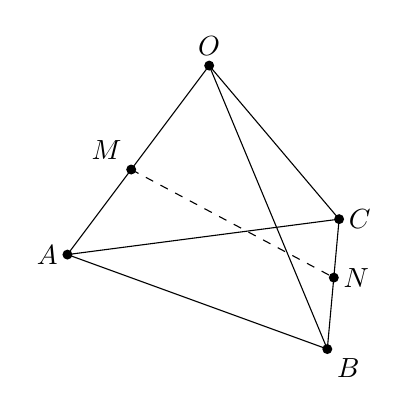
\begin{tikzpicture}[scale=1.5,baseline=(current bounding box.north)]
		\coordinate (A) at (-1.2,0);
		\coordinate (B) at (1,-0.8);
		\coordinate (C) at (1.1,0.3);
		\coordinate (O) at (0,1.6);
		\coordinate (M) at ($(A)!0.45!(O)$);
		\coordinate (N) at ($(B)!0.55!(C)$);
		\draw (A)--(B)--(C)--cycle;
		\draw (O)--(A); \draw (O)--(B); \draw (O)--(C);
		\draw[dashed] (M)--(N);
		\fill (A) circle (1.2pt) node[left] {$A$};
		\fill (B) circle (1.2pt) node[below right] {$B$};
		\fill (C) circle (1.2pt) node[right] {$C$};
		\fill (O) circle (1.2pt) node[above] {$O$};
		\fill (M) circle (1.2pt) node[above left] {$M$};
		\fill (N) circle (1.2pt) node[right] {$N$};
	\end{tikzpicture}
\end{minipage}

\category{向量共面}
\begin{question}
	已知$\overrightarrow{p}=2\overrightarrow{a}-\overrightarrow{b}+2\overrightarrow{c},\quad
	\overrightarrow{q}=-\overrightarrow{a}+3\overrightarrow{b}-3\overrightarrow{c},\quad
	\overrightarrow{r}=13\overrightarrow{a}+6\overrightarrow{b}+\lambda\overrightarrow{c}
	$若$\overrightarrow{p},\overrightarrow{q},\overrightarrow{r}$共面，则$\lambda=$?
\end{question}
三向量共面：
\[
13\overrightarrow{a}+6\overrightarrow{b}+\lambda\overrightarrow{c}=x\left(2\overrightarrow{a}-\overrightarrow{b}+2\overrightarrow{c}\right)+y\left(-\overrightarrow{a}+3\overrightarrow{b}-3\overrightarrow{c}\right)
\]
整理右侧：
\[
13\overrightarrow{a}+6\overrightarrow{b}+\lambda\overrightarrow{c}
=(2x-y)\overrightarrow{a}+(-x+3y)\overrightarrow{b}+(2x-3y)\overrightarrow{c}
\]
由向量相等，对应系数相等建立方程组：
\[
\begin{cases}
	2x-y=13\\
	-x+3y=6\\
	\lambda=2x-3y
\end{cases}
\]
解得：$x=9,\;y=5$，代入得 $\lambda=3$.

\category{四点共面}
\begin{question}{}
	$A,B,C,D$四点共面，且$\overrightarrow{DP}=m\overrightarrow{OA}+\overrightarrow{OB}+\overrightarrow{OC}$，求$m=$？
\end{question}
四点共面结论：起点一样，则向量系数之和为$1$.
\[
\begin{aligned}
	\overrightarrow{OP}-\overrightarrow{OB}&=m\overrightarrow{OA}+\overrightarrow{OB}+\overrightarrow{OC} \\
	\overrightarrow{OP}&=m\overrightarrow{OA}+2\overrightarrow{OB}+\overrightarrow{OC}
\end{aligned}
\]
\[
m+2+1=1 \implies m=-2
\]

\subsubsection{向量的数量积}
\begin{knowledge}{投影相关公式}
	投影：$|\overrightarrow{b}|\cdot\cos\langle\overrightarrow{a},\overrightarrow{b}\rangle$
	
	投影向量：$\displaystyle |\overrightarrow{b}|\cdot\cos\langle\overrightarrow{a},\overrightarrow{b}\rangle\cdot\frac{\overrightarrow{a}}{|\overrightarrow{a}|}$
\end{knowledge}

\begin{question}{}
	已知$AB=4,AD=3,AA'=3$，$\angle BAD=90^\circ$，$\angle BAA'=60^\circ$，$\angle DAA'=60^\circ$，求$|AC'|$.
\end{question}

\begin{minipage}[t]{0.5\textwidth}
	\[
	\begin{aligned}
		|\overrightarrow{AC'}|&=\sqrt{(\overrightarrow{AB}+\overrightarrow{AD}+\overrightarrow{AA'})^2} \\
		&=\sqrt{|\overrightarrow{AB}|^2+|\overrightarrow{AD}|^2+|\overrightarrow{AA'}|^2
			+2\overrightarrow{AB}\cdot\overrightarrow{AD}+2\overrightarrow{AD}\cdot\overrightarrow{AA'}+2\overrightarrow{AB}\cdot\overrightarrow{AA'}} \\
		&=\sqrt{4^2+3^2+3^2+0+9+12} \\
		&=\sqrt{55}
	\end{aligned}
	\]
\end{minipage}
\hfill
\begin{minipage}[t]{0.3\textwidth}
	\centering
	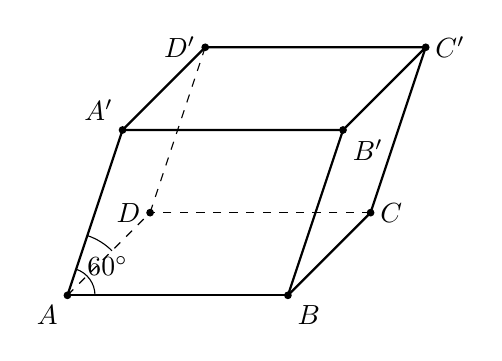
\begin{tikzpicture}[scale=0.7,baseline=(current bounding box.north)]
		% 命名点
		\coordinate (A) at (0,0);
		\coordinate (B) at (4,0);
		\coordinate (C) at (5.5,1.5);
		\coordinate (D) at (1.5,1.5);
		\coordinate (A') at (1,3);
		\coordinate (B') at (5,3);
		\coordinate (C') at (6.5,4.5);
		\coordinate (D') at (2.5,4.5);
		
		% 用括号括起所有坐标名
		\draw[thick] (A) -- (B);
		\draw[thick] (B) -- (C);
		\draw[dashed] (A) -- (D);
		\draw[dashed] (C) -- (D);
		\draw[thick] (A') -- (B') -- (C') -- (D') -- cycle;
		\draw[thick] (A) -- (A');
		\draw[thick] (B) -- (B');
		\draw[thick] (C) -- (C');
		\draw[dashed] (D) -- (D');
		
		% 批量标记所有点
		\foreach \p/\pos in {A/below left,B/below right,C/right,D/left,A'/above left,B'/below right,C'/right,D'/left}
		\fill (\p) circle (2pt) node[\pos] {$\p$};
		\draw pic["$60^\circ$", draw, angle eccentricity=1.8, angle radius=0.35cm] 
		{angle = B--A--A'};
		\draw pic["", draw, angle eccentricity=2.5, angle radius=0.8cm] 
		{angle = D--A--A'};
	\end{tikzpicture}
\end{minipage}

\subsubsection{坐标运算}
\begin{question}{}
	若$A(m+1,n+1,3),\,B(2m,n,m-2n),\,C(m+3,n-3,9)$三点共线，则$m+n=$？
\end{question}
\[
\overrightarrow{AB}=(m-1,-1,m-2n-3),\quad \overrightarrow{AC}=(2,-4,6)
\]
三点共线：$\overrightarrow{AB}=\lambda\overrightarrow{AC}$，由$y$分量可知 $\lambda=\dfrac{1}{4}$.
\[
\begin{cases}
	\dfrac{2}{4}=m-1 \\
	\dfrac{6}{4}=m-2n-3
\end{cases}
\implies
\begin{cases}
	m=\dfrac{3}{2}\\[4pt]
	n=-\dfrac{3}{2}
\end{cases}
\implies m+n=0
\]

\begin{question}
	已知点$A(2,-1,7)$，向量$\overrightarrow{a}=(18,9,-12)$，$\overrightarrow{AB}\parallel\overrightarrow{a}$，线段长$|AB|=34$，求$B$点坐标.
\end{question}

$\overrightarrow{AB}\parallel\overrightarrow{a}\implies \overrightarrow{AB}=\lambda\overrightarrow{a}\ (\lambda>0)$

设$B(x,y,z)$

$(x-2,y+1,z-7)=\lambda(18,9,-12)$

$\sqrt{(18\lambda)^2+(9\lambda)^2+(-12\lambda)^2}=34 \implies \lambda=2$

$\therefore B=(38,17,-17)$

\subsection{第二讲\quad 立体几何中的向量方法}

\subsubsection{方向向量与法向量}
\begin{knowledge}{基本定义}
	直线的方向向量：$A,B$ 为直线上不同两点，则与 $\overrightarrow{AB}$ 平行的向量称为直线的方向向量.
	
	平面的法向量：若 $\boldsymbol{n}\perp$ 平面，则与 $\boldsymbol{n}$ 平行的非零向量为平面法向量.
\end{knowledge}

\begin{knowledge}{法向量标准求解步骤}
	\begin{enumerate}[label=\bfseries\arabic*.]
		\item 建立空间直角坐标系，写出点坐标；
		\item 求出平面内两条相交边对应的方向向量；
		\item 设法向量 $\boldsymbol{n}=(x,y,z)$，列数量积为0的方程组；
		\item 赋值，解方程组得到一组法向量.
	\end{enumerate}
\end{knowledge}
以一点为原点，三条两两垂直的方向分别作为坐标轴，建立空间直角坐标系.

\category{正方体求法向量}
\begin{question}
	正方体棱长为3，设 $A(3,0,0),\,E(3,3,1),\,F(0,3,2)$，求平面$AEF$的一个法向量.
\end{question}
\begin{minipage}[t]{0.5\textwidth}
	$\overrightarrow{AE}=(0,3,1),\quad \overrightarrow{FE}=(3,0,-1)$
	
	设平面$AEF$的一个法向量为 $\boldsymbol{n}=(x,y,z)$，满足
	\[
	\begin{cases}
		\boldsymbol{n}\cdot\overrightarrow{AE}=0\\
		\boldsymbol{n}\cdot\overrightarrow{FE}=0
	\end{cases}
	\implies
	\begin{cases}
		3y+z=0\\
		3x-z=0
	\end{cases}
	\]
	令 $z=3$，得 $x=1,\,y=-1$，可取 $\boldsymbol{n}=(1,-1,3)$.
\end{minipage}
\hfill
\begin{minipage}[t]{0.34\textwidth}
	\tdplotsetmaincoords{70}{110}
	\begin{tikzpicture}[baseline=(current bounding box.north), scale=1
		,tdplot_main_coords
		]
		% 坐标点定义
		\coordinate (D) at (0,0,0);
		\coordinate (A) at (3,0,0);
		\coordinate (B) at (3,3,0);
		\coordinate (C) at (0,3,0);
		\coordinate (D1) at (0,0,3);
		\coordinate (A1) at (3,0,3);
		\coordinate (B1) at (3,3,3);
		\coordinate (C1) at (0,3,3);
		
		% 三等分点 E 和 F
		\coordinate (E) at (3,3,1); % E 在 BB1 上
		\coordinate (F) at (0,3,2); % F 在 CC1 上
		
		% 坐标轴 (内部虚线，外部实线)
		\draw[->, dashed] (D) -- (A);
		\draw[->, thick] (A) -- (4.5,0,0) node[below] {$x$};
		\draw[->, dashed] (D) -- (C);
		\draw[->, thick] (C) -- (0,4.5,0) node[right] {$y$};
		\draw[->, dashed] (D) -- (D1);
		\draw[->, thick] (D1) -- (0,0,4.5) node[above] {$z$};
		
		% 正方体可见边
		\draw[thick] (A) -- (B) -- (C);
		\draw[thick] (A) -- (A1);
		\draw[thick] (B) -- (B1);
		\draw[thick] (C) -- (C1);
		\draw[thick] (A1) -- (B1) -- (C1) -- (D1) -- cycle;
		
		% 顶点标签
		\node[left] at (A) {$A$};
		\node[right] at (B) {$B$};
		\node[below right] at (C) {$C$};
		\node[left] at (D) {$D$};
		\node[left] at (A1) {$A_1$};
		\node[right] at (B1) {$B_1$};
		\node[above right] at (C1) {$C_1$};
		\node[left] at (D1) {$D_1$};
		
		% 平面 AEF (可见边界为实线，不可见为虚线)
		\draw[thick, dashed] (A) -- (F); % 穿过体内部
		\draw[thick] (A) -- (E);         % 前面
		\draw[thick] (E) -- (F);         % 右侧面
		
		% 标注 E, F 点
		\node[right] at (E) {$E$};
		\node[right] at (F) {$F$};
		\fill (E) circle (1.5pt);
		\fill (F) circle (1.5pt);
	\end{tikzpicture}
\end{minipage}

\subsubsection{空间平行、垂直与空间向量的关系}

\begin{knowledge}{平行、垂直判定结论}
	\begin{itemize}
		\item 线$\parallel$线 $\iff$ 方向向量互相平行；线$\perp$线 $\iff$ 方向向量互相垂直
		\item 线$\parallel$面 $\iff$ 直线方向向量与平面法向量垂直；线$\perp$面 $\iff$ 直线方向向量与平面法向量平行
		\item 面$\parallel$面 $\iff$ 两平面法向量互相平行；面$\perp$面 $\iff$ 两平面法向量互相垂直
	\end{itemize}
	
	可画图确认
\end{knowledge}

\category{正方体证明线面垂直}
\begin{question}{正方体线面平行证明}
	正方体，$E$为$BC$中点，$F$为$CD$中点，$G$为$C_1D_1$中点，求证：$BG\parallel$ 平面$EFC_1$.
\end{question}
\begin{minipage}[t]{0.7\textwidth}
	设正方体棱长为$2$，以$C$为原点，$CB,CD,CC_1$分别为$x,y,z$轴建系：
	\[
	C(0,0,0), B(2,0,0), D(0,2,0), C_1(0,0,2), D_1(0,2,2)
	\]
	\[
	E(1,0,0), F(0,1,0), G(0,1,2)
	\]
	\[
	\overrightarrow{FE}=(1,-1,0), \overrightarrow{FC_1}=(0,-1,2)
	\]
	设平面$EFC_1$法向量$\boldsymbol{n}=(x,y,z)$
	\[
	\begin{cases}
		\boldsymbol{n}\cdot\overrightarrow{FE}=x-y=0\\
		\boldsymbol{n}\cdot\overrightarrow{FC_1}=-y+2z=0
	\end{cases}
	\Rightarrow x=y=2z,\text{取}z=1,\boldsymbol{n}=(2,2,1)
	\]
	\[
	\overrightarrow{BG}=(-2,1,2)
	\]
	\[
	\overrightarrow{BG}\cdot\boldsymbol{n}=2\times(-2)+2\times1+1\times2=0
	\]
	又$BG\not\subset$平面$EFC_1$，故$BG\parallel$平面$EFC_1$.
\end{minipage}
\hfill
\begin{minipage}[t]{0.34\textwidth}
	\tdplotsetmaincoords{70}{110}
	\begin{tikzpicture}[baseline=(current bounding box.north), scale=1.5,tdplot_main_coords]
		\coordinate (C) at (0,0,0);
		\coordinate (B) at (2,0,0);
		\coordinate (D) at (0,2,0);
		\coordinate (A) at (2,2,0);
		\coordinate (C1) at (0,0,2);
		\coordinate (B1) at (2,0,2);
		\coordinate (D1) at (0,2,2);
		\coordinate (A1) at (2,2,2);
		\coordinate (E) at (1,0,0);
		\coordinate (F) at (0,1,0);
		\coordinate (G) at (0,1,2);
		
		\draw[->, dashed] (C)--(B);
		\draw[->, thick] (B)--(3,0,0) node[below]{$x$};
		\draw[->, dashed] (C)--(D);
		\draw[->, thick] (D)--(0,3,0) node[right]{$y$};
		\draw[->, dashed] (C)--(C1);
		\draw[->, thick] (C1)--(0,0,3) node[above]{$z$};
		
		\draw[thick] (A)--(B)--(C)--(D)--cycle;
		\draw[thick] (A1)--(B1)--(C1)--(D1)--cycle;
		\draw[thick] (A)--(A1) (B)--(B1) (D)--(D1);
		\draw[thick, SkyBlue] (E)--(F)--(C1)--cycle;
		\draw[thick, red] (B)--(G);
		
		\node[below right] at (A) {$A$};
		\node[left] at (B) {$B$};
		\node[left] at (C) {$C$};
		\node[below] at (D) {$D$};
		\node[right] at (A1) {$A_1$};
		\node[left] at (B1) {$B_1$};
		\node[left] at (C1) {$C_1$};
		\node[right] at (D1) {$D_1$};
		\fill (E) circle (1.5pt) node[below]{$E$};
		\fill (F) circle (1.5pt) node[below left]{$F$};
		\fill (G) circle (1.5pt) node[above left]{$G$};
	\end{tikzpicture}
\end{minipage}

\subsubsection{角度问题}
\begin{knowledge}{三类空间角向量公式}
	\begin{itemize}
		\item 线线角：$\cos\theta=\left|\cos\langle \overrightarrow{v_1},\overrightarrow{v_2}\rangle\right|$
		\item 线面角：$\sin\theta=\left|\cos\langle \overrightarrow{v},\boldsymbol{n}\rangle\right|$，$\overrightarrow{v}$ 为直线方向向量，$\boldsymbol{n}$ 为平面法向量
		\item 面面角：$|\cos\theta|=\left|\cos\langle \boldsymbol{n_1},\boldsymbol{n_2}\rangle\right|$，$\boldsymbol{n_1},\boldsymbol{n_2}$ 为两平面法向量
	\end{itemize}
\end{knowledge}

\category{长方体求线面角}
\begin{question}
	$AB=AA_1=2, AD=4$, $M$是$A_1B_1$中点
	
	(1) $BC$与平面$BMD_1$是所成角的正弦值
	
	(2) $\angle B-MD_1-B_1$的余弦值
\end{question}

\begin{minipage}[t]{0.5\textwidth}
	\begin{enumerate}[label=(\arabic*)]
		\item $\overrightarrow{BC}$的方向向量为$\overrightarrow{v}=(0,1,0)$
		
		$\overrightarrow{n}=(4,1,-2)$
		
		$\sin \theta =|cos\langle\overrightarrow{v},\overrightarrow{n}\rangle|=\dfrac{\sqrt{21}}{21}$
		\item $\overrightarrow{n}'=(0,0,1)$
		
		$|\cos\theta| = |\cos\langle\overrightarrow{n},\overrightarrow{n}'\rangle|=\dfrac{2\sqrt{21}}{21}$
		
		$\therefore \angle B-MD_1-B_1$的余弦值为$\dfrac{2\sqrt{21}}{21}$ 
	\end{enumerate}
	
	
\end{minipage}
\hfill
\begin{minipage}[t]{0.4\textwidth}
	\tdplotsetmaincoords{70}{110}
	\begin{tikzpicture}[baseline=(current bounding box.north), scale=1,tdplot_main_coords]
		% 长方体坐标，A在上，A1在下，AB=2, AA1=2, AD=4
		\coordinate (A) at (0,0,2);
		\coordinate (B) at (2,0,2);
		\coordinate (D) at (0,4,2);
		\coordinate (C) at (2,4,2);
		\coordinate (A1) at (0,0,0);
		\coordinate (B1) at (2,0,0);
		\coordinate (D1) at (0,4,0);
		\coordinate (C1) at (2,4,0);
		% M 为 A1B1 中点
		\coordinate (M) at ($(A1)!0.5!(B1)$);
		
		% 坐标轴
		\draw[->, dashed] (A1) -- (B1);
		\draw[->, thick] (B1) -- (3,0,0) node[below] {$x$};
		\draw[->, dashed] (A1) -- (D1);
		\draw[->, thick] (D1) -- (0,5,0) node[right] {$y$};
		\draw[->, dashed] (A1) -- (A);
		\draw[->, thick] (A) -- (0,0,3) node[above] {$z$};
		
		% 长方体棱 实线可见
		\draw[thick] (A)--(B)--(C)--(D)--cycle;
		\draw[thick] (A1)--(B1)--(C1)--(D1)--cycle;
		\draw[thick] (A)--(A1);
		\draw[thick] (B)--(B1);
		\draw[thick] (C)--(C1);
		\draw[thick] (D)--(D1);
		
		% 目标平面 BMD1 线条
		\draw[thick] (B)--(M);
		\draw[thick] (M)--(D1);
		\draw[thick] (B)--(D1);
		\draw[thick] (M)--(B1);
		
		% 顶点标注
		\node[above left] at (A) {$A$};
		\node[above left] at (B) {$B$};
		\node[above] at (D) {$D$};
		\node[above] at (C) {$C$};
		\node[above left] at (A1) {$A_1$};
		\node[left] at (B1) {$B_1$};
		\node[below] at (D1) {$D_1$};
		\node[below] at (C1) {$C_1$};
		\node[left] at (M) {$M$};
		
		% 标记特殊点
		\fill (M) circle (1.5pt);
	\end{tikzpicture}
\end{minipage}

\subsection{第三讲\quad 直线方程}
\subsubsection{直线方程}
\begin{knowledge}{直线方程（五类方程）}
	倾斜角：$l$向上方向与$x$正方向夹角
	斜率 $k=\tan\alpha=\dfrac{y_2-y_1}{x_2-x_1}$
	
	技巧：注意$k>0$是否在题目范围内；倾斜角需要分类讨论
	\begin{enumerate}[label=\bfseries\arabic*.]
		\item 点斜式方程：$y-y_0=k(x-x_0)$ \quad[一个点+ $k$] \quad \textbf{不能表示垂直$x$轴直线}
		\item 斜截式方程：$y=kx+b$，$b$为纵截距 \quad [纵截距+ $k$] \quad \textbf{不能表示$\alpha=90^\circ$}
		\item 两点式方程 \quad [求$k$+点斜式]
		\item 截距式方程：过$(a,0)$和$(0,b)$，$\dfrac{x}{a}+\dfrac{y}{b}=1$
		\quad \textbf{不能表示横、竖直线，不能表示过原点直线}
		\item 一般式方程 $Ax+By+C=0$（不轻易用）
	\end{enumerate}
\end{knowledge}

\category{关于截距}
\begin{question}
	经过$(1,2)$且两截距绝对值相等的直线方程为?
\end{question}
题目涉及截距，优先考虑截距式，分类讨论：
\begin{enumerate}[label=\arabic*.]
	\item 直线过原点：$y=2x$
	\item 直线不过原点，不是横竖直线
	\begin{enumerate}[label=(\arabic*)]
		\item $a=b$，$\dfrac{x}{a}+\dfrac{y}{a}=1$，代入$(1,2)$，得$a=3$，方程：$x+y-3=0$
		\item $a=-b$，$\dfrac{x}{a}-\dfrac{y}{a}=1$，代入$(1,2)$，得$a=-1$，方程：$-x+y=1$
	\end{enumerate}
\end{enumerate}

\subsubsection{位置关系与距离公式}
\begin{knowledge}{位置关系与距离公式}
	对于一般式 $A_1x+B_1y+C_1=0,\ A_2x+B_2y+C_2=0$
	\begin{itemize}
		\item 平行：$\dfrac{A_1}{A_2}=\dfrac{B_1}{B_2}\neq\dfrac{C_1}{C_2}$，注意排除重合直线
		\item 垂直：$A_1A_2+B_1B_2=0$
	\end{itemize}
	
	点到直线距离：$\displaystyle d=\dfrac{|Ax_0+By_0+C|}{\sqrt{A^2+B^2}}$
	
	两平行线距离：$\displaystyle d=\dfrac{|C_1-C_2|}{\sqrt{A^2+B^2}}$
	先将$x,y$系数统一再求C！
	
	圆锥曲线大题意识：看到带参数的直线方程，表明直线过定点.
\end{knowledge}

\category{直线平行判定}
\begin{question}
	设$m\in\mathbb{R}$，则$m=-3$是直线$mx+3y=2-m$与$x+(m+1)y=1$平行的什么条件？
\end{question}
平行条件：$\dfrac{A_1}{A_2}=\dfrac{B_1}{B_2}\neq\dfrac{C_1}{C_2}$
\[
\dfrac{m}{1}=\dfrac{3}{m+1}\implies m=-3 \text{ 或 }m=2
\]
当$m=2$时，两条直线方程相同，为重合，舍去.\newline
故为充要条件.

\category{点线距}
\begin{question}
	直线过$(-1,2)$，原点到直线距离为$1$，求直线方程
\end{question}
\begin{enumerate}[label=\arabic*.]
	\item 直线垂直$x$轴：$x=-1$
	\item 直线不垂直$x$轴，设斜率$k$
	\[
	y-2=k(x+1)\implies kx-y+k+2=0
	\]
	\[
	d=\dfrac{|k+2|}{\sqrt{k^2+1}}=1,\quad |k+2|=\sqrt{k^2+1}
	\]
	解得 $k=-\dfrac{3}{4}$，直线方程：$3x+4y-5=0$
\end{enumerate}

\category{线线距}
\begin{question}
	两条平行直线$3x+4y-12=0$与$ax+8y+11=0$之间的距离为?
\end{question}
平行直线满足：$\dfrac{3}{a}=\dfrac{4}{8}$，解得$a=6$.
前提：$A,B$系数统一，第一个方程左右同乘$2$：$6x+8y-24=0$，此时$A=6,B=8,C_1=-24,C_2=11$.
\[
d=\dfrac{|-24-11|}{\sqrt{6^2+8^2}}=\dfrac{35}{10}=\dfrac{7}{2}.
\]

\category{斜率取值范围}
\begin{question}
	过原点的直线$l$的倾斜角取值范围为$\left[\dfrac{\pi}{3},\dfrac{3\pi}{4}\right]$，则其斜率的取值范围?
\end{question}
\begin{minipage}[t]{0.5\textwidth}
	$\tan\dfrac{\pi}{3}=\sqrt{3},\ \tan\dfrac{3\pi}{4}=-1$.
	
	由图像可得斜率范围：$(-\infty,-1]\cup[\sqrt{3},+\infty)$.
\end{minipage}
\begin{minipage}[t]{0.45\textwidth}
	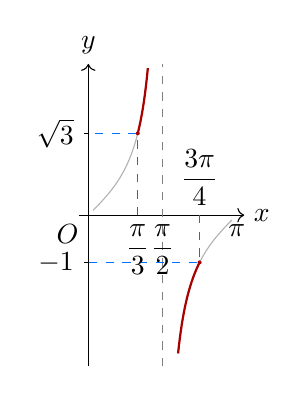
\begin{tikzpicture}[scale=0.6,baseline=(current bounding box.north)]
		\draw[->] (-0.2,0)--(3.3,0) node[right]{$x$};
		\draw[->] (0,-3.2)--(0,3.2) node[above]{$y$};
		
		% 仅标记关键y值
		\draw (0,-1)--(-0.1,-1) node[left] {$-1$};
		\draw (0,{sqrt(3)})--(-0.1,{sqrt(3)}) node[left] {$\sqrt{3}$};
		
		% tanx 只画 [0, pi] 一个周期，远离pi/2渐近线
		\draw[gray!60] plot[domain=0.1:1.26] (\x,{tan(deg(\x))});
		\draw[gray!60] plot[domain=1.9:3.04] (\x,{tan(deg(\x))});
		
		%目标区间红线
		\draw[DarkRed,thick] plot[domain={pi/3}:1.26] (\x,{tan(deg(\x))});
		\draw[DarkRed,thick] plot[domain=1.9:{3*pi/4}] (\x,{tan(deg(\x))});
		
		%渐近线虚线 x=π/2
		\draw[dashed,gray] (pi/2,-3.2)--(pi/2,3.2);
		
		%辅助虚线
		\draw[dashed,SkyBlue] (pi/3,0)--(pi/3,{sqrt(3)})--(0,{sqrt(3)});
		\draw[dashed,SkyBlue] (3*pi/4,0)--(3*pi/4,-1)--(0,-1);
		
		%关键点标记
		\fill[DarkRed] (pi/3,{sqrt(3)}) circle (1.2pt);
		\fill[DarkRed] (3*pi/4,-1) circle (1.2pt);
		
		%刻度，3π/4保留above避免图像遮挡
		\node[below] at (pi/3,0) {$\dfrac{\pi}{3}$};
		\node[below] at (pi/2,0) {$\dfrac{\pi}{2}$};
		\node[above] at (3*pi/4,0) {$\dfrac{3\pi}{4}$};
		\node[below] at (pi,0) {$\pi$};
		\node[below left] at (0,0) {$O$};
	\end{tikzpicture}
\end{minipage}

\category{过定点}
\begin{question}
	$(2k-1)x-(k+3)y-(k-11)=0$过定点?
\end{question}
整理式子：
\[
k(2x-y-1)-x-3y+11=0
\]
联立方程组
\[
\begin{cases}
	2x-y-1=0\\
	-x-3y+11=0
\end{cases}
\]
解得$\begin{cases}x=2\\y=3\end{cases}$，直线过定点$(2,3)$.

\subsection{第四讲\quad 直线与圆}
\category{圆的方程、点、线、圆与圆的位置关系}

\subsubsection{圆的方程}
\begin{knowledge}{}
	以$(a,b)$为圆心、$r$为半径的圆的标准方程：
	\[
	(x-a)^2+(y-b)^2=r^2
	\]
	圆心坐标：$(a,b)$.
	
	圆的一般方程：$x^2+y^2+Dx+Ey+F=0$
	\begin{enumerate}
		\item $x^2$、$y^2$项系数相等且不为$0$；
		\item 圆心坐标为$\left(-\dfrac{D}{2},-\dfrac{E}{2}\right)$，半径为$\dfrac12\sqrt{D^2+E^2-4F}$；
		\item 只有$x^2$、$y^2$系数为$1$，才可直接读取参数$D,E,F$；
		\item $D^2+E^2-4F>0$，方程才表示圆.
	\end{enumerate}
	已知圆上三点，可列三元一次方程组求解圆方程.
\end{knowledge}

\subsubsection{点、直线、圆与圆的位置关系}
\begin{knowledge}{}
	\begin{enumerate}
		\item 点与圆：将点代入圆方程，结果与$r^2$比较大小.
		\item 直线与圆
		\begin{enumerate}
			\item 计算圆心到直线距离，与半径比较；
			\item 联立直线与圆方程，消元得到一元二次方程，通过判别式$\Delta$判定位置.
		\end{enumerate}
		\item 圆与圆：计算两圆圆心距，和$|r_1-r_2|$、$r_1+r_2$比较.
	\end{enumerate}
	内含：$d<|r_1-r_2|$；内切：$d=|r_1-r_2|$；
	
	相交：$|r_1-r_2|<d<r_1+r_2$；外切：$d=r_1+r_2$；外离：$d>r_1+r_2$.
\end{knowledge}

\begin{question}{例题1}
	方程$a^2x^2+(a+2)y^2+4x+8y+5a=0$表示圆，求该圆的圆心.
\end{question}
解：
圆方程中$x^2,y^2$系数相等
\[
a^2 = a+2 \implies a=2 \text{ 或 } a=-1
\]
当$a=2$，代入得
\[
4x^2+4y^2+4x+8y+10=0
\]
\[
x^2+y^2+x+2y+\frac52=0
\]
$D^2+E^2-4F<0$，不表示圆，舍去.

当$a=-1$，满足条件，圆心为$(-2,-4)$.

\vspace{6pt}
\begin{question}{例题2}
	直线$3x+4y+m=0$与圆$x^2+y^2-2x+4y+1=0$相切，求$m$的值.
\end{question}
圆$x^2+y^2-2x+4y+1=0$圆心$(1,-2)$，半径$r=2$.
\[
d=\frac{|3-8+m|}{5}=2 \implies m=-5 \text{ 或 } m=15
\]

\vspace{6pt}
\begin{question}{例题3}
	半径为$\sqrt2$，且与圆$x^2+y^2+10x+10y=0$外切于原点，求该圆的标准方程.
\end{question}
\begin{minipage}[t]{0.7\textwidth}
	解：
	圆$x^2+y^2+10x+10y=0$圆心$(-5,-5)$，半径$5\sqrt2$.
	两圆外切于原点，则所求圆圆心在直线$y=x$上，设圆心$(m,m)$.
	\[
	\sqrt{2(m+5)^2}=6\sqrt2 \implies m=1
	\]
	圆心$(1,1)$，半径$\sqrt2$.
	\[
	(x-1)^2+(y-1)^2=2
	\]
\end{minipage}
\begin{minipage}[t]{0.3\textwidth}
	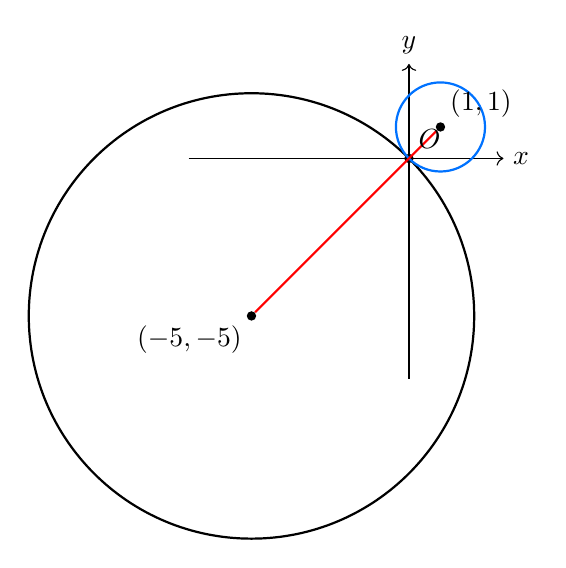
\begin{tikzpicture}[scale=0.4,baseline=(current bounding box.north)]
		\draw[->](-7,0)--(3,0) node[right]{$x$};
		\draw[->](0,-7)--(0,3) node[above]{$y$};
		\coordinate[circle,fill,inner sep=1.2pt] (Oa) at (-5,-5);
		\coordinate[circle,fill,inner sep=1.2pt] (Ob) at (1,1);
		\coordinate[circle,fill,inner sep=1.2pt] (O) at (0,0);
		\draw[thick] (Oa) circle({5*sqrt(2)});
		\draw[thick,SkyBlue] (Ob) circle({sqrt(2)});
		\draw[thick,red] (Oa)--(Ob);
		\node[below left] at (Oa) {$(-5,-5)$};
		\node[above right] at (Ob) {$(1,1)$};
		\node[above right] at (O) {$O$};
	\end{tikzpicture}
\end{minipage}

\begin{knowledge}{弦长公式}
	弦长$l=2\sqrt{r^2-d^2}$，其中$d$为圆心到直线的距离
\end{knowledge}

\category{弦长问题}
\begin{question}
	过$A(11,2)$作圆$x^2+y^2+2x-4y-164=0$的弦，弦长为整数的共有几个？
\end{question}

\begin{minipage}[t]{0.7\textwidth}
	圆方程配方：$(x+1)^2+(y-2)^2=169$，圆心$O(-1,2)$，半径$r=13$.
	
	点$A(11,2)$到圆心距离：$|OA|=\sqrt{(11+1)^2+(2-2)^2}=12<r$，故点在圆内.
	
	最短弦长（垂直于$OA$）：$l_{\min}=2\sqrt{13^2-12^2}=2\sqrt{25}=10$
	
	最长弦长（直径）：$l_{\max}=2r=26$
	
	弦长取值范围：$[10,26]$，整数弦长有$10,11,12,\cdots,26$共$17$个值.
	
	\begin{enumerate}[label=\arabic*.]
		\item 弦长为$10$（最短弦）：只有$1$条
		\item 弦长为$26$（直径）：只有$1$条
		\item 弦长为$11,12,\cdots,25$：共$15$个值，由圆的对称性，每个值对应$2$条弦
	\end{enumerate}
	
	合计：$1+1+15\times2=32$条.
\end{minipage}
\hfill
\begin{minipage}[t]{0.3\textwidth}
	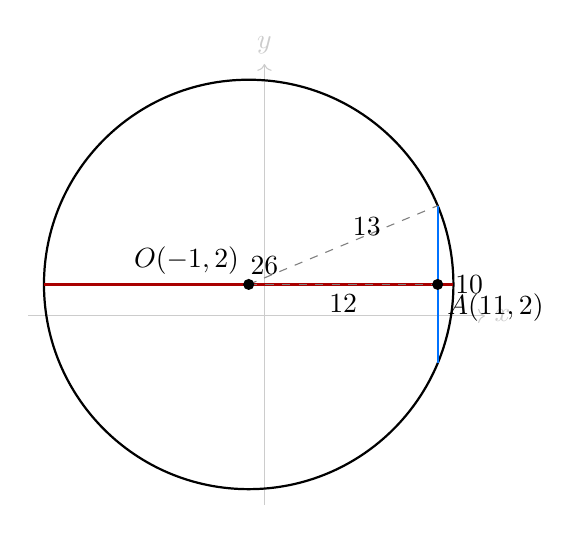
\begin{tikzpicture}[scale=0.2,baseline=(current bounding box.north)]
		\coordinate (O) at (-1,2);
		\coordinate (A) at (11,2);
		\coordinate (shortTop) at (11,7);
		\coordinate (shortBot) at (11,-3);
		\coordinate (longLeft) at (-14,2);
		\coordinate (longRight) at (12,2);
		
		% 坐标轴
		\draw[->,gray!40] (-15,0) -- (14,0) node[right] {$x$};
		\draw[->,gray!40] (0,-12) -- (0,16) node[above] {$y$};
		
		% 圆
		\draw[thick] (O) circle (13);
		
		% 最长弦（直径，红色）
		\draw[thick,DarkRed] (longLeft) -- (longRight);
		
		% 最短弦（蓝色，垂直于OA）
		\draw[thick,SkyBlue] (shortBot) -- (shortTop);
		
		% 辅助虚线：OA
		\draw[dashed,gray] (O) -- (A);
		
		% 辅助虚线：半径到最短弦端点
		\draw[dashed,gray] (O) -- (shortTop);
		
		% 标点
		\fill (O) circle (10pt) node[above left] {$O(-1,2)$};
		\fill (A) circle (10pt) node[below right] {$A(11,2)$};
		
		% 标注
		\node[above] at (0,2) {$26$};
		\node[right] at (11.5,2) {$10$};
		\node[below] at (5,2) {$12$};
		\node[above right] at (5,4.5) {$13$};
	\end{tikzpicture}
\end{minipage}

\subsection{第五讲\quad 椭圆初步}

\subsubsection{椭圆的定义}
\begin{knowledge}{椭圆的定义}
	与两定点$F_1,F_2$的距离的和为常数（大于$|F_1F_2|$）的轨迹叫椭圆.
	\[
	\begin{aligned}
		|MF_1|+|MF_2| &> |F_1F_2|=2c \quad \text{椭圆} \\
		|MF_1|+|MF_2| &= |F_1F_2|=2c \quad \text{线段} \\
		|MF_1|+|MF_2| &< |F_1F_2|=2c \quad \text{不存在}
	\end{aligned}
	\]
\end{knowledge}

\category{代数求方程}
\begin{question}
	已知椭圆$\dfrac{x^2}{a^2}+\dfrac{y^2}{b^2}=1$的焦点为$(3,0)$，且$a=2b$，求椭圆的方程.
\end{question}
\begin{enumerate}[label=\arabic*.]
	\item 焦点位置：$x$轴
	\item 两个条件：$\begin{cases} a=2b \\ a^2=b^2+c^2 \end{cases}$，焦点$(3,0)\implies c=3$
\end{enumerate}
$\therefore a=2\sqrt{3},\ b=\sqrt{3},\ c=3$，椭圆方程：$\dfrac{x^2}{12}+\dfrac{y^2}{3}=1$.

\subsubsection{椭圆的标准方程}
\begin{knowledge}{标准方程}
	\[
	\frac{x^2}{a^2}+\frac{y^2}{b^2}=1 \qquad a^2=b^2+c^2
	\]
	\textbf{判断焦点位置：}谁的分母大，焦点在谁那，谁就是$a^2$.
\end{knowledge}

\category{代数求方程}
\begin{question}
	椭圆过定点$(3,0)$且$a=3b$，求标准方程.
\end{question}
过$(3,0)$并不是焦点，需分类讨论：
\begin{enumerate}[label=\arabic*.]
	\item 焦点在$x$轴：$\dfrac{x^2}{a^2}+\dfrac{y^2}{b^2}=1$.
	\newline $\because (3,0)$有个$0$，很特殊，代入$\dfrac{9}{a^2}=1\implies a=3,\ b=1$.
	\newline $\therefore \dfrac{x^2}{9}+y^2=1$.
	\item 焦点在$y$轴：$\dfrac{y^2}{a^2}+\dfrac{x^2}{b^2}=1$.
	\newline 将$(3,0)$代入$\dfrac{9}{b^2}=1\implies b=3,\ a=9$.
	\newline $\therefore \dfrac{y^2}{81}+\dfrac{x^2}{9}=1$.
\end{enumerate}

\subsubsection{几何性质}
\begin{knowledge}{几何性质}
	\begin{minipage}[t]{0.7\textwidth}
		\begin{itemize}
			\item 离心率：$e=\dfrac{c}{a}=\sqrt{1-\dfrac{b^2}{a^2}}=\sqrt{\dfrac{c^2}{b^2+c^2}}$等，平方再开根.
			\newline \textbf{性质：}$e$越大越扁.
			\item 通径：$|MN|=\dfrac{2b^2}{a}$（用$a^2=b^2+c^2$换值）.
		\end{itemize}
		
		\begin{knowledge}{求离心率的方法}
			\begin{enumerate}[label=\arabic*.]
				\item 找到$a,b,c$（初学）.
				\item 焦点三角形法（两焦点+一点在椭圆上）.
				\item 几何关系找到$a,b,c$等式.
			\end{enumerate}
		\end{knowledge}
		
		
		\begin{minipage}[t]{0.7\textwidth}
			\textbf{方法2举例：}
			
			在椭圆中，设$|PF_1|=7x, |PF_2|=3x$
			
			则$|F_1F_2|=2c=5x$.
			
			由椭圆定义：$|PF_1|+|PF_2|=2a=7x+3x=10x$.
			
			$\therefore e=\dfrac{c}{a}=\dfrac{5x}{10x}=\dfrac{1}{2}$.
		\end{minipage}
		\hfill
		\begin{minipage}[t]{0.2\textwidth}
			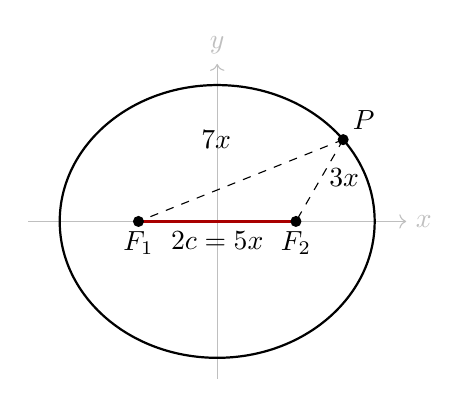
\begin{tikzpicture}[scale=0.2, baseline=(current bounding box.north)]
				\coordinate (F1) at (-5,0);
				\coordinate (F2) at (5,0);
				\coordinate (P) at (8, {sqrt(27)});
				\draw[->, gray!50] (-12,0) -- (12,0) node[right] {$x$};
				\draw[->, gray!50] (0,-10) -- (0,10) node[above] {$y$};
				\draw[thick] (0,0) ellipse (10 and {sqrt(75)});
				\draw[dashed] (P) -- (F1);
				\draw[dashed] (P) -- (F2);
				\draw[thick, DarkRed] (F1) -- (F2);
				\fill (F1) circle (10pt) node[below] {$F_1$};
				\fill (F2) circle (10pt) node[below] {$F_2$};
				\fill (P) circle (10pt) node[above right] {$P$};
				\node[below] at (0,0) {$2c=5x$};
				\node[above left] at (1.5,4) {$7x$};
				\node[below right] at (6.5,4) {$3x$};
			\end{tikzpicture}
		\end{minipage}
		
		\vspace{6pt}
		\textbf{方法3举例：}
		\begin{enumerate}[label=\arabic*.]
			\item 若$b=c$：
			\[
			e=\frac{c}{a}=\sqrt{\frac{c^2}{a^2}}=\sqrt{\frac{c^2}{b^2+c^2}}=\sqrt{\frac{1}{2}}=\frac{\sqrt{2}}{2}
			\]
			\item 若$b^2=ac$：
			\[
			a^2-c^2=ac \xrightarrow{\text{同除}a^2} 1-e^2=e
			\]
		\end{enumerate}
	\end{minipage}
	\hfill
	\begin{minipage}[t]{0.3\textwidth}
		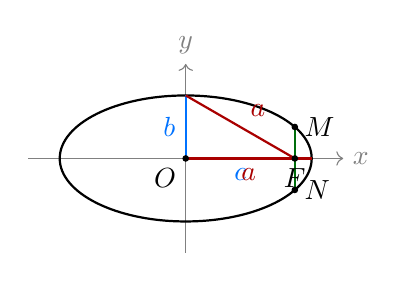
\begin{tikzpicture}[scale=0.8,baseline=(current bounding box.north)]
			\draw[->,gray] (-2.5,0) -- (2.5,0) node[right] {$x$};
			\draw[->,gray] (0,-1.5) -- (0,1.5) node[above] {$y$};
			\draw[thick] (0,0) ellipse (2 and 1);
			\coordinate (O) at (0,0);
			\coordinate (A) at (2,0);
			\coordinate (B) at (0,1);
			\coordinate (F) at ({sqrt(3)},0);
			\coordinate (M) at ({sqrt(3)},0.5);
			\coordinate (N) at ({sqrt(3)},-0.5);
			
			\draw[thick, SkyBlue] (O) -- (B) node[midway, left] {$b$};
			\draw[thick, SkyBlue] (O) -- (F) node[midway, below] {$c$};
			\draw[thick, DarkRed] (B) -- (F) node[midway, above right] {$a$};
			\draw[thick, DarkRed] (O) -- (A) node[midway, below] {$a$};
			\draw[thick, DarkGreen] (M) -- (N);
			
			\fill (O) circle (1.5pt) node[below left] {$O$};
			\fill (F) circle (1.5pt) node[below] {$F$};
			\fill (M) circle (1.5pt) node[right] {$M$};
			\fill (N) circle (1.5pt) node[right] {$N$};
		\end{tikzpicture}
	\end{minipage}
\end{knowledge}

\category{代数求方程}
\begin{question}
	过$(3,2)$且与椭圆$3x^2+8y^2=24$有相同焦点，求椭圆方程.
\end{question}
化简已知椭圆：$\dfrac{x^2}{8}+\dfrac{y^2}{3}=1$，焦点在$x$轴，$c^2=8-3=5$.

\textbf{A方法（待定系数法）：}
设椭圆方程为$\dfrac{x^2}{b^2+5}+\dfrac{y^2}{b^2}=1$.
代入$(3,2)$：
\[
\frac{9}{b^2+5}+\frac{4}{b^2}=1 \implies 9b^2+4(b^2+5)=b^2(b^2+5)
\]
\[
b^4-8b^2-20=0 \implies (b^2-10)(b^2+2)=0
\]
$\because b^2>0, \therefore b^2=10, a^2=15$.
方程为$\dfrac{x^2}{15}+\dfrac{y^2}{10}=1$.

\vspace{6pt}
\textbf{B方法（定义法）：}
\begin{minipage}[t]{0.65\textwidth}
	焦点$F_1(-\sqrt{5},0), F_2(\sqrt{5},0)$. 由定义 $|MF_1|+|MF_2|=2a$.
	\[
	2a = \sqrt{(3+\sqrt{5})^2+2^2} + \sqrt{(3-\sqrt{5})^2+2^2}
	\]
	\[
	2a = \sqrt{18+6\sqrt{5}} + \sqrt{18-6\sqrt{5}}
	\]
	两边平方：
	\[
	4a^2 = (18+6\sqrt{5}) + (18-6\sqrt{5}) + 2\sqrt{(18+6\sqrt{5})(18-6\sqrt{5})}
	\]
	\[
	4a^2 = 36 + 2\sqrt{324-180} = 36 + 24 = 60
	\]
	$\therefore a^2=15, b^2=a^2-c^2=10$.
	方程为$\dfrac{x^2}{15}+\dfrac{y^2}{10}=1$.
\end{minipage}
\hfill
\begin{minipage}[t]{0.35\textwidth}
	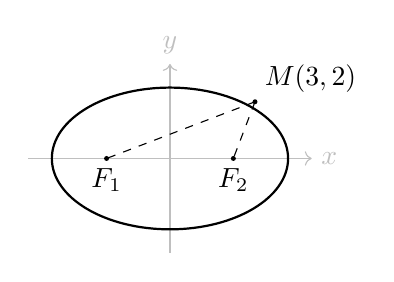
\begin{tikzpicture}[scale=0.6, baseline=(current bounding box.north)]
		\draw[->, gray!50] (-3,0) -- (3,0) node[right] {$x$};
		\draw[->, gray!50] (0,-2) -- (0,2) node[above] {$y$};
		\draw[thick] (0,0) ellipse (2.5 and 1.5);
		\coordinate (F1) at ({-sqrt(5)*0.6}, 0);
		\coordinate (F2) at ({sqrt(5)*0.6}, 0);
		\coordinate (M) at (1.8, 1.2);
		
		\draw[dashed] (M) -- (F1);
		\draw[dashed] (M) -- (F2);
		
		\fill (F1) circle (1.5pt) node[below] {$F_1$};
		\fill (F2) circle (1.5pt) node[below] {$F_2$};
		\fill (M) circle (1.5pt) node[above right] {$M(3,2)$};
	\end{tikzpicture}
\end{minipage}

\category{代数求方程}
\begin{question}
	椭圆$x^2+my^2=1$的焦点在$y$轴上，长轴是短轴的$2$倍，$m=$?
\end{question}
化为标准方程：$\dfrac{x^2}{1}+\dfrac{y^2}{1/m}=1$.
焦点在$y$轴，故$a^2=\dfrac{1}{m}, b^2=1$.
由$a=2b$：
\[
a=\sqrt{\frac{1}{m}}=2\times 1=2 \implies m=\frac{1}{4}.
\]

\category{离心率求方程}
\begin{question}
	椭圆离心率$e=\dfrac{\sqrt{3}}{2}$，过点$(2,1)$，$\dfrac{x^2}{a^2}+\dfrac{y^2}{b^2}=1\ (a>b>0)$，求方程.
\end{question}
\[
e=\frac{\sqrt{3}}{2}=\sqrt{\frac{a^2-b^2}{a^2}} \implies a^2=4b^2
\]
将$(2,1)$代入$\dfrac{x^2}{a^2}+\dfrac{y^2}{b^2}=1$：
\[
\frac{4}{4b^2}+\frac{1}{b^2}=1 \implies b^2=2,\ a^2=8.
\]
椭圆方程：$\dfrac{x^2}{8}+\dfrac{y^2}{2}=1$.

\category{几何求方程}
\begin{question}
	已知椭圆$\dfrac{x^2}{a^2}+\dfrac{y^2}{b^2}=1\ (a>b>0)$，$F_1,F_2$为焦点，$AB$在椭圆上，$AB\perp F_1F_2$于$F_2$，$|AB|=4$，$|F_1F_2|=2\sqrt{3}$，求方程.
\end{question}
\begin{minipage}[t]{0.7\textwidth}
	$|F_1F_2|=2c=2\sqrt{3} \implies c=\sqrt{3}$.
	
	$AB$为通径：$|AB|=\dfrac{2b^2}{a}=4 \implies b^2=2a$.
	
	又$b^2=a^2-c^2=a^2-3$，故：
	\[
	2a=a^2-3 \implies a^2-2a-3=0 \implies a=3.
	\]
	$\therefore b^2=6$.
	
	椭圆方程：$\dfrac{x^2}{9}+\dfrac{y^2}{6}=1$.
\end{minipage}
\hfill
\begin{minipage}[t]{0.3\textwidth}
	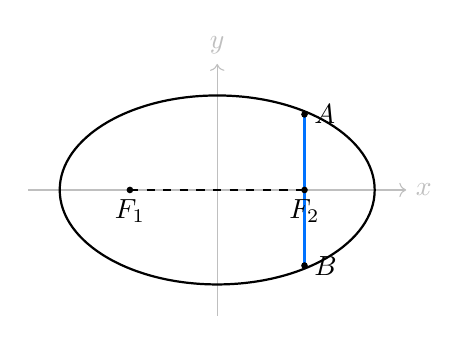
\begin{tikzpicture}[scale=0.8, baseline=(current bounding box.north)]
		\draw[->, gray!50] (-3,0) -- (3,0) node[right] {$x$};
		\draw[->, gray!50] (0,-2) -- (0,2) node[above] {$y$};
		\draw[thick] (0,0) ellipse (2.5 and 1.5);
		\coordinate (F1) at ({-sqrt(3)*0.8}, 0);
		\coordinate (F2) at ({sqrt(3)*0.8}, 0);
		\coordinate (A) at ({sqrt(3)*0.8}, 1.2);
		\coordinate (B) at ({sqrt(3)*0.8}, -1.2);
		
		\draw[thick, SkyBlue] (A) -- (B);
		\draw[dashed] (F1) -- (F2);
		
		\fill (F1) circle (1.5pt) node[below] {$F_1$};
		\fill (F2) circle (1.5pt) node[below] {$F_2$};
		\fill (A) circle (1.5pt) node[right] {$A$};
		\fill (B) circle (1.5pt) node[right] {$B$};
	\end{tikzpicture}
\end{minipage}

\category{找$a,b,c$求离心率}
\begin{question}
	已知椭圆$C:\dfrac{x^2}{a^2}+\dfrac{y^2}{4}=1\ (a>2)$，直线$l:y=x-2$过$C$的一个焦点，求$C$的离心率.
\end{question}
$\because a>2$，$\therefore$ 焦点在$x$轴上.

令$y=0$，得$x=2$，即焦点为$(2,0)$.

$\therefore c=2,\ b=2,\ a=\sqrt{b^2+c^2}=2\sqrt{2}$.

\[
e=\frac{c}{a}=\frac{2}{2\sqrt{2}}=\frac{\sqrt{2}}{2}.
\]

\category{焦点三角形法求离心率}
\begin{question}
	已知椭圆$\dfrac{x^2}{a^2}+\dfrac{y^2}{b^2}=1$左右焦点为$F_1,F_2$，$P$为椭圆上一点，且$\angle PF_1F_2=30^\circ$，$\angle PF_2F_1=60^\circ$，离心率=?
\end{question}

\begin{minipage}[t]{0.6\textwidth}
	在$\triangle PF_1F_2$中，$\angle F_1PF_2 = 180^\circ - 30^\circ - 60^\circ = 90^\circ$.
	
	设$|F_1F_2|=2c$.
	
	$|PF_2| = 2c \cdot \sin30^\circ = c$.
	
	$|PF_1| = 2c \cdot \cos30^\circ = \sqrt{3}c$.
	
	由定义 $|PF_1|+|PF_2|=2a$:
	
	$2a = \sqrt{3}c + c = (\sqrt{3}+1)c$.
	
	$\therefore e = \dfrac{2c}{2a} = \dfrac{2}{\sqrt{3}+1} = \sqrt{3}-1$.
\end{minipage}
\hfill
\begin{minipage}[t]{0.4\textwidth}
	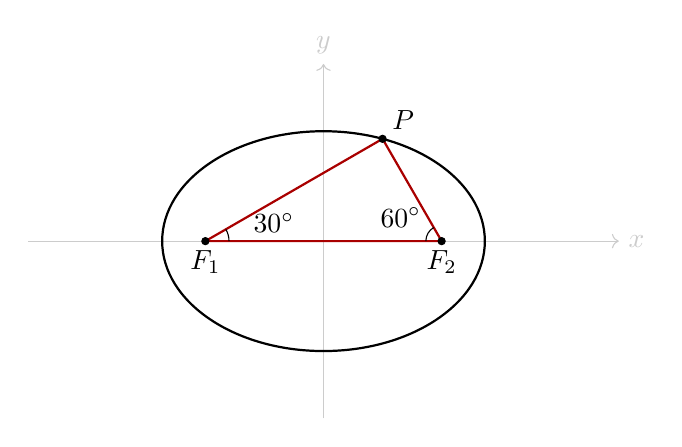
\begin{tikzpicture}[scale=1.5, baseline=(current bounding box.north)]
		\pgfmathsetmacro{\c}{1}
		\pgfmathsetmacro{\a}{(sqrt(3)+1)/2}
		\pgfmathsetmacro{\b}{sqrt(\a*\a - \c*\c)}
		
		\draw[->, gray!40] (-2.5,0) -- (2.5,0) node[right] {$x$};
		\draw[->, gray!40] (0,-1.5) -- (0,1.5) node[above] {$y$};
		
		\draw[thick] (0,0) ellipse (\a cm and \b cm);
		
		\coordinate (F1) at (-\c, 0);
		\coordinate (F2) at (\c, 0);
		\coordinate (P) at (0.5, {\c*sqrt(3)/2});
		
		\draw[thick, DarkRed] (F1) -- (P) -- (F2) -- cycle;
		
		\fill (F1) circle (1pt) node[below] {$F_1$};
		\fill (F2) circle (1pt) node[below] {$F_2$};
		\fill (P) circle (1pt) node[above right] {$P$};
		
		\draw pic["$30^\circ$", draw, angle eccentricity=3, angle radius=0.3cm] {angle = F2--F1--P};
		\draw pic["$60^\circ$", draw, angle eccentricity=3, angle radius=0.2cm] {angle = P--F2--F1};
	\end{tikzpicture}
\end{minipage}

\vspace{10pt}

\category{几何关系求离心率}
\begin{question}
	$PF_1$中点在$y$轴上，若$\angle PF_1F_2=30^\circ$，离心率=?
\end{question}

\begin{minipage}[t]{0.7\textwidth}
	设$PF_1$中点为$M$，$O$为原点（即$F_1F_2$中点）.
	
	$\therefore OM$为$\triangle PF_1F_2$的中位线
	
	$\therefore OM \parallel PF_2$.
	
	$\because M$在$y$轴上
	
	$\therefore OM \perp F_1F_2$（$x$轴）.
	
	$\therefore PF_2 \perp F_1F_2$，即$\triangle PF_1F_2$为直角三角形.
	
	设$|PF_2|=1$.
	
	$\because \angle PF_1F_2=30^\circ$
	
	$\therefore |PF_1|=2, |F_1F_2|=\sqrt{3}$.
	
	$2c = |F_1F_2| = \sqrt{3} \implies c=\dfrac{\sqrt{3}}{2}$.
	
	$2a = |PF_1|+|PF_2| = 2+1=3 \implies a=\dfrac{3}{2}$.
	
	$\therefore e = \dfrac{c}{a} = \dfrac{\frac{\sqrt{3}}{2}}{\frac{3}{2}} = \dfrac{\sqrt{3}}{3}$.
\end{minipage}
\hfill
\begin{minipage}[t]{0.3\textwidth}
	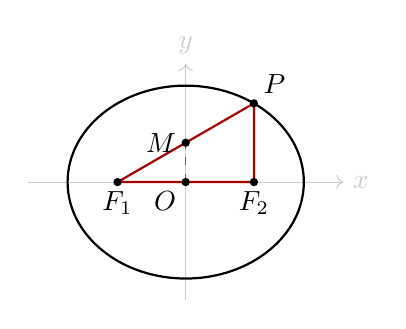
\begin{tikzpicture}[scale=0.5, baseline=(current bounding box.north)]
		\pgfmathsetmacro{\c}{sqrt(3)}
		\pgfmathsetmacro{\a}{3}
		\pgfmathsetmacro{\b}{sqrt(6)}
		
		\draw[->, gray!40] (-4,0) -- (4,0) node[right] {$x$};
		\draw[->, gray!40] (0,-3) -- (0,3) node[above] {$y$};
		
		\draw[thick] (0,0) ellipse (\a cm and \b cm);
		
		\coordinate (F1) at (-\c, 0);
		\coordinate (F2) at (\c, 0);
		\coordinate (O) at (0,0);
		\coordinate (P) at (\c, 2);
		\coordinate (M) at ($(F1)!0.5!(P)$);
		
		\draw[thick, DarkRed] (F1) -- (P) -- (F2) -- cycle;
		\draw[dashed, SkyBlue] (O) -- (M);
		
		\fill (F1) circle (3pt) node[below] {$F_1$};
		\fill (F2) circle (3pt) node[below] {$F_2$};
		\fill (O) circle (3pt) node[below left] {$O$};
		\fill (P) circle (3pt) node[above right] {$P$};
		\fill (M) circle (3pt) node[left] {$M$};
	\end{tikzpicture}
\end{minipage}

\subsection{第六讲\quad 双曲线初步}

\subsubsection{双曲线的定义}
\begin{knowledge}{双曲线的定义}
	与两定点$F_1,F_2$距离之差的绝对值等于常数(小于$|F_1F_2|$)的点的轨迹叫双曲线.
	\[
	\begin{aligned}
		||MF_1|-|MF_2|| &= 2a < |F_1F_2|=2c \quad \text{双曲线} \\
		||MF_1|-|MF_2|| &= 2a = |F_1F_2|=2c \quad \text{两条射线} \\
		||MF_1|-|MF_2|| &= 2a > |F_1F_2|=2c \quad \text{不存在}
	\end{aligned}
	\]
	不加绝对值为双曲线的一支(一条射线,不存在对应上).
	
	\textbf{注意：}$c$是老大.
\end{knowledge}

\category{焦点+点}
\begin{question}
	与双曲线$\dfrac{x^2}{16}-\dfrac{y^2}{4}=1$有相同焦点,且经过$(3\sqrt{2},2)$的双曲线标准方程?
\end{question}

$a^2=16, b^2=4, c^2=20=a^2+b^2$.

设所求方程为$\dfrac{x^2}{a^2}-\dfrac{y^2}{b^2}=1 \implies \dfrac{x^2}{20-b^2}-\dfrac{y^2}{b^2}=1$.

代入$(3\sqrt{2},2)$:
\[
\frac{18}{20-b^2}-\frac{4}{b^2}=1 \implies 18b^2-4(20-b^2)=b^2(20-b^2)
\]

通分整理：$b^4+2b^2-80=0 \implies (b^2+10)(b^2-8)=0$.

$\because b^2>0$

$\therefore b^2=8, a^2=12$.

$\therefore$ 方程为$\dfrac{x^2}{12}-\dfrac{y^2}{8}=1$.


\subsubsection{双曲线的标准方程}
\begin{knowledge}{标准方程}
	$\dfrac{x^2}{a^2}-\dfrac{y^2}{b^2}=1$ 或 $\dfrac{y^2}{a^2}-\dfrac{x^2}{b^2}=1$.
	谁的系数正,焦点在谁上($a^2$).
	
	一般式$mx^2+ny^2=1$:
	\begin{enumerate}[label=\arabic*.]
		\item $m=n>0$ 圆
		\item $m\neq n>0$ 椭圆
		\item $m\cdot n<0$ 双曲线
		\item $m<0,n<0$ 不存在
	\end{enumerate}
\end{knowledge}


\begin{question}
	若方程$\dfrac{x^2}{1+k}+\dfrac{y^2}{1-k}=1$表示双曲线,$k$范围?
\end{question}

$(1+k)(1-k)<0 \implies k \in (-\infty,-1)\cup(1,+\infty)$.

\category{点+渐近线}
\begin{question}
	已知双曲线过点$(1,\sqrt{2})$且渐近线为$y=\pm\sqrt{3}x$,方程?
\end{question}
\begin{minipage}[t]{0.7\textwidth}
	点+渐近线才可判断焦点位置.
	
	将$x=1$代入$y=\sqrt{3}x$中,$y=\sqrt{3}>\sqrt{2}$,过$x$轴.
	
	分析渐近线:$\sqrt{3}=\dfrac{b}{a}$.
	
	\textbf{A方法:} $\dfrac{x^2}{a^2}-\dfrac{y^2}{(\sqrt{3}a)^2}=1$
	
	代入$(1,\sqrt{2}) \implies a^2=\dfrac{1}{3}, b^2=1$.
	
	\textbf{B方法:} 共渐近线,写出$\sqrt{3}a=b$的方程:$x^2-\dfrac{y^2}{3}=\lambda$.
	
	代入$(1,\sqrt{2}) \implies \lambda=\dfrac{1}{3}$.
	
	$\therefore 3x^2-y^2=1$.
\end{minipage}
\hfill
\begin{minipage}[t]{0.3\textwidth}
	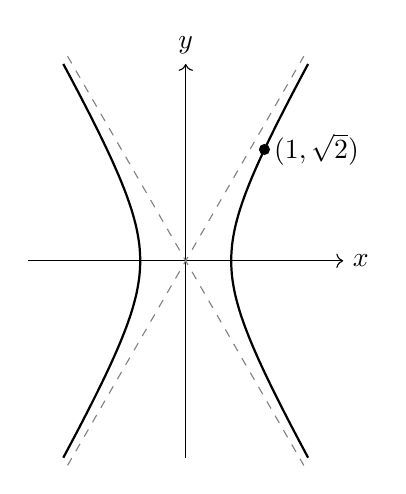
\begin{tikzpicture}[scale=1, baseline=(current bounding box.north)]
		\draw[->, black] (-2,0) -- (2,0) node[right] {$x$};
		\draw[->, black] (0,-2.5) -- (0,2.5) node[above] {$y$};
		
		\draw[thick, domain=-2.5:2.5, smooth, variable=\y] plot ({sqrt((\y*\y+1)/3)}, \y);
		\draw[thick, domain=-2.5:2.5, smooth, variable=\y] plot ({-sqrt((\y*\y+1)/3)}, \y);
		
		% 渐近线
		\draw[dashed, gray] (-1.5,{-1.5*sqrt(3)}) -- (1.5,{1.5*sqrt(3)});
		\draw[dashed, gray] (-1.5,{1.5*sqrt(3)}) -- (1.5,{-1.5*sqrt(3)});
		
		% 标点
		\fill (1,{sqrt(2)}) circle (2pt) node[right] {$(1,\sqrt{2})$};
	\end{tikzpicture}
\end{minipage}

\subsubsection{几何性质}
\begin{knowledge}{几何性质}
	\begin{minipage}[t]{0.7\textwidth}
		
		实轴为$2a$
		
		渐近线$y=\pm\dfrac{b}{a}x$(焦点在$x$轴)或$y=\pm\dfrac{a}{b}x$(焦点在$y$轴).
		
		类比斜率$\dfrac{y_F}{x_F}$.
	\end{minipage}
	\hfill
	\begin{minipage}[t]{0.3\textwidth}
	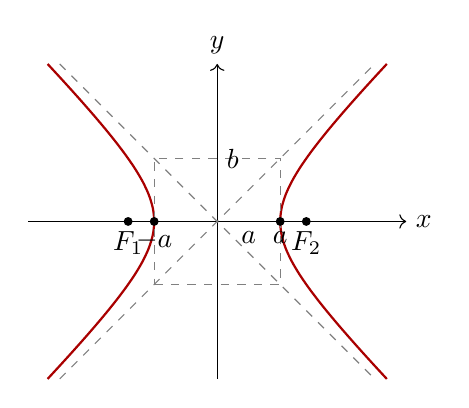
\begin{tikzpicture}[scale=0.8, baseline=(current bounding box.north)]
		% 坐标轴（黑色）
		\draw[->, black] (-3,0) -- (3,0) node[right] {$x$};
		\draw[->, black] (0,-2.5) -- (0,2.5) node[above] {$y$};
		
		% 双曲线
		\draw[thick, DarkRed, domain=-2.5:2.5, smooth, variable=\y] plot ({sqrt(1+\y*\y)}, \y);
		\draw[thick, DarkRed, domain=-2.5:2.5, smooth, variable=\y] plot ({-sqrt(1+\y*\y)}, \y);
		
		% 渐近线
		\draw[dashed, gray] (-2.5,-2.5) -- (2.5,2.5);
		\draw[dashed, gray] (-2.5,2.5) -- (2.5,-2.5);
		
		% 辅助矩形
		\draw[dashed, gray] (-1,-1) -- (1,-1) -- (1,1) -- (-1,1) -- cycle;
		
		% 坐标点
		\coordinate (F1) at (-{sqrt(2)},0);
		\coordinate (F2) at ({sqrt(2)},0);
		\coordinate (A1) at (-1,0);
		\coordinate (A2) at (1,0);
		
		% 标点
		\fill (F1) circle (2pt) node[below] {$F_1$};
		\fill (F2) circle (2pt) node[below] {$F_2$};
		\fill (A1) circle (2pt) node[below] {$-a$};
		\fill (A2) circle (2pt) node[below] {$a$};
		
		% 标注 a 和 b
		\node[right] at (0,1) {$b$};
		\node[below] at (0.5,0) {$a$};
	\end{tikzpicture}
	\end{minipage}
\end{knowledge}

\category{渐近线(多解)}
\begin{question}
	实轴为6,渐近线$y=\pm\dfrac{3}{2}x$的双曲线方程?
\end{question}

$2a=6, a=3$.
\begin{enumerate}[label=\arabic*.]
	\item 焦点在$x$轴:$\dfrac{b}{a}=\dfrac{3}{2} \implies a=3 \implies b=\dfrac{9}{2} \implies \dfrac{x^2}{9}-\dfrac{y^2}{\frac{81}{4}}=1$.
	\item 焦点在$y$轴:$\dfrac{a}{b}=\dfrac{3}{2} \implies a=3 \implies b=2 \implies \dfrac{y^2}{9}-\dfrac{x^2}{4}=1$.
\end{enumerate}

\category{焦点+共渐近线}
\begin{question}
	和椭圆$\dfrac{x^2}{49}+\dfrac{y^2}{24}=1$共焦点，和双曲线$\dfrac{x^2}{36}-\dfrac{y^2}{64}=1$共渐近线的双曲线方程？
\end{question}

椭圆中 $a^2=49, b^2=24 \implies c^2=25$，焦点在$x$轴.

双曲线渐近线斜率 $\dfrac{b}{a} = \sqrt{\dfrac{64}{36}} = \dfrac{4}{3}$.

设所求双曲线方程为 $\dfrac{x^2}{9\lambda} - \dfrac{y^2}{16\lambda} = 1\ (\lambda>0)$.

\[
c^2 = 9\lambda + 16\lambda = 25\lambda = 25 \implies \lambda=1.
\]
方程为 $\dfrac{x^2}{9} - \dfrac{y^2}{16} = 1$.

\category{通径}
\begin{question}
	过双曲线$\dfrac{x^2}{a^2}-\dfrac{y^2}{b^2}=1$的一个焦点作实轴的垂线，交双曲线于$A,B$两点，$|AB|=$实轴长，求离心率.
\end{question}

通径长 $|AB| = \dfrac{2b^2}{a}$.

由题意 $\dfrac{2b^2}{a} = 2a \implies a=b$.

\[
e = \frac{c}{a} = \sqrt{\frac{a^2+b^2}{a^2}} = \sqrt{2}.
\]

\category{焦点三角形}
\begin{question}
	焦点在$x$轴的双曲线，$P$为双曲线右支上一点，$\triangle OPF_2$为正三角形（$O$为原点，$F_2$为右焦点），求离心率.
\end{question}

\begin{minipage}[t]{0.7\textwidth}
	$\because \triangle OPF_2$ 为正三角形
	
	$\therefore |OP|=|OF_2|=|PF_2|=c$.
	
	在 $\triangle PF_1F_2$ 中，$|OP| = \dfrac{1}{2}|F_1F_2| = c$
	
	$\therefore \triangle PF_1F_2$ 为直角三角形，$\angle F_1PF_2 = 90^\circ$.
	
	\[
	|PF_2| = c, \quad |PF_1| = \sqrt{|F_1F_2|^2 - |PF_2|^2} = \sqrt{3}c.
	\]
	
	由定义 $|PF_1| - |PF_2| = 2a$:
	\[
	\sqrt{3}c - c = 2a \implies e = \frac{2c}{2a} = \frac{2}{\sqrt{3}-1} = \sqrt{3}+1.
	\]
\end{minipage}
\hfill
\begin{minipage}[t]{0.3\textwidth}
	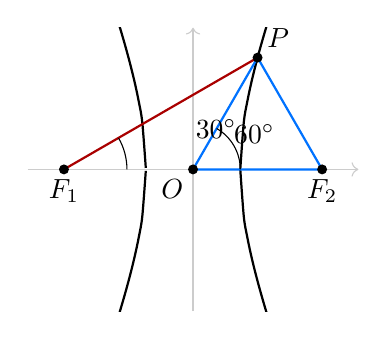
\begin{tikzpicture}[scale=0.6, baseline=(current bounding box.north)]
		\pgfmathsetmacro{\a}{1}
		\pgfmathsetmacro{\c}{sqrt(3)+1}
		\pgfmathsetmacro{\b}{sqrt(\c*\c - \a*\a)}
		\pgfmathsetmacro{\px}{\c/2}
		\pgfmathsetmacro{\py}{sqrt(3)*\c/2}
		
		% 先裁剪超出范围的部分
		\clip (-3.5,-3) rectangle (3.5,3);
		
		\draw[->, gray!40] (-3.5,0) -- (3.5,0) node[right] {$x$};
		\draw[->, gray!40] (0,-3) -- (0,3) node[above] {$y$};
		
		% 使用题目推导出的准确参数绘图，确保P在曲线上
		% 限制domain避免曲线太长
		\draw[thick, domain=1:2.8, smooth, variable=\x] plot ({\x}, {\b*sqrt(\x*\x-1)/\a});
		\draw[thick, domain=1:2.8, smooth, variable=\x] plot ({\x}, {-\b*sqrt(\x*\x-1)/\a});
		\draw[thick, domain=-2.8:-1, smooth, variable=\x] plot ({\x}, {\b*sqrt(\x*\x-1)/\a});
		\draw[thick, domain=-2.8:-1, smooth, variable=\x] plot ({\x}, {-\b*sqrt(\x*\x-1)/\a});
		
		\coordinate (F1) at (-\c, 0);
		\coordinate (F2) at (\c, 0);
		\coordinate (O) at (0,0);
		\coordinate (P) at (\px, \py);
		
		\draw[thick, SkyBlue] (O) -- (P) -- (F2) -- cycle;
		\draw[thick, DarkRed] (F1) -- (P);
		
		\fill (F1) circle (3pt) node[below] {$F_1$};
		\fill (F2) circle (3pt) node[below] {$F_2$};
		\fill (O) circle (3pt) node[below left] {$O$};
		\fill (P) circle (3pt) node[above right] {$P$};
		
		\draw pic["$30^\circ$", draw, angle eccentricity=2.5, angle radius=0.8cm] {angle = F2--F1--P};
		\draw pic["$60^\circ$", draw, angle eccentricity=1.5, angle radius=0.6cm] {angle = F2--O--P};
	\end{tikzpicture}
\end{minipage}

\category{几何关系}
\begin{question}
	焦点在$x$轴，直线$x=c$与双曲线渐近线交$A,B$，若$\triangle F_1AB$为等腰直角三角形（$F_1$为左焦点），求离心率.
\end{question}
\begin{minipage}[t]{0.7\textwidth}
	直线 $x=c$ 过右焦点 $F_2(c,0)$ 且垂直于 $x$ 轴.
	
	$A, B$ 在渐近线 $y=\pm\dfrac{b}{a}x$ 上
	
	$\therefore A(c, \dfrac{bc}{a}), B(c, -\dfrac{bc}{a})$.
	
	$\because \triangle F_1AB$ 为等腰直角三角形，且 $F_1F_2 \perp AB$
	
	$\therefore \angle AF_1F_2 = 45^\circ \implies |F_1F_2| = |AF_2|$.
	\[
	2c = \frac{bc}{a} \implies b=2a.
	\]
	\[
	e = \sqrt{1+\left(\frac{b}{a}\right)^2} = \sqrt{1+4} = \sqrt{5}.
	\]
\end{minipage}
\hfill
\begin{minipage}[t]{0.3\textwidth}
	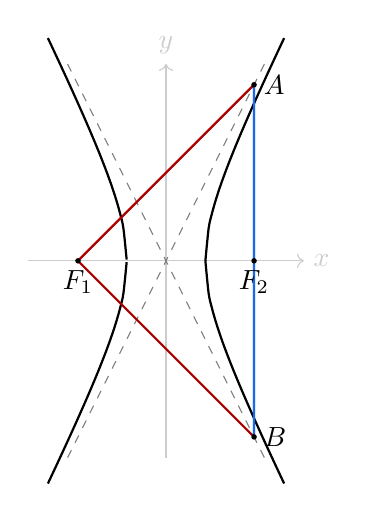
\begin{tikzpicture}[scale=0.5, baseline=(current bounding box.north)]
		\pgfmathsetmacro{\a}{1}
		\pgfmathsetmacro{\b}{2}
		\pgfmathsetmacro{\c}{sqrt(5)}
		
		% 坐标轴
		\draw[->, gray!40] (-3.5,0) -- (3.5,0) node[right] {$x$};
		\draw[->, gray!40] (0,-5) -- (0,5) node[above] {$y$};
		
		% 双曲线 x^2 - y^2/4 = 1
		\draw[thick, domain=1:3, smooth, variable=\x] plot ({\x}, {\b*sqrt(\x*\x-1)/\a});
		\draw[thick, domain=1:3, smooth, variable=\x] plot ({\x}, {-\b*sqrt(\x*\x-1)/\a});
		\draw[thick, domain=-3:-1, smooth, variable=\x] plot ({\x}, {\b*sqrt(\x*\x-1)/\a});
		\draw[thick, domain=-3:-1, smooth, variable=\x] plot ({\x}, {-\b*sqrt(\x*\x-1)/\a});
		
		% 渐近线 y = ±2x (斜率修正为 2)
		\draw[dashed, gray] (-2.5,-5) -- (2.5,5);
		\draw[dashed, gray] (-2.5,5) -- (2.5,-5);
		
		% 坐标点
		\coordinate (F1) at (-\c, 0);
		\coordinate (F2) at (\c, 0);
		% A, B 在渐近线上，x=c 时 y = ±(b/a)*c = ±2*sqrt(5)
		\coordinate (A) at (\c, {\b*\c/\a}); 
		\coordinate (B) at (\c, {-\b*\c/\a});
		
		% 连线
		\draw[thick, DarkRed] (F1) -- (A) -- (B) -- cycle;
		\draw[thick, SkyBlue] (A) -- (B);
		
		% 标点
		\fill (F1) circle (2pt) node[below] {$F_1$};
		\fill (F2) circle (2pt) node[below] {$F_2$};
		\fill (A) circle (2pt) node[right] {$A$};
		\fill (B) circle (2pt) node[right] {$B$};
	\end{tikzpicture}
\end{minipage}

\category{两次焦点三角形}
\begin{question}
	$P$在左支，$PF_2$和右支交点为$Q$，若$\triangle PF_1Q$为等边三角形，求离心率.
\end{question}

\begin{minipage}[t]{0.7\textwidth}
	两个焦点三角形：$\triangle PF_1F_2, \triangle QF_1F_2$.
	
	$\triangle PF_1F_2$: $PF_2 - PF_1 = 2a$.
	
	$\because \triangle PF_1Q$ 为等边三角形
	
	$\therefore PF_1 = F_1Q = PQ = x$.
	
	又 $P, Q, F_2$ 共线
	
	$\therefore PF_2 = PQ + QF_2 = x + QF_2$.
	
	$\therefore QF_2 = PF_2 - PF_1 = 2a$.
	
	$\triangle QF_1F_2$: $QF_1 - QF_2 = 2a$.
	
	$\therefore x - 2a = 2a \implies x = 4a$.
	
	在 $\triangle PF_1F_2$ 中，$\angle F_1PF_2 = 60^\circ$.
	
	由余弦定理：
	\[
	F_1F_2^2 = PF_1^2 + PF_2^2 - 2PF_1 \cdot PF_2 \cdot \cos 60^\circ
	\]
	\[
	4c^2 = (4a)^2 + (6a)^2 - 2(4a)(6a) \cdot \frac{1}{2} = 28a^2
	\]
	
	$\therefore c = \sqrt{7}a, e = \sqrt{7}$.
\end{minipage}
\hfill
\begin{minipage}[t]{0.3\textwidth}
	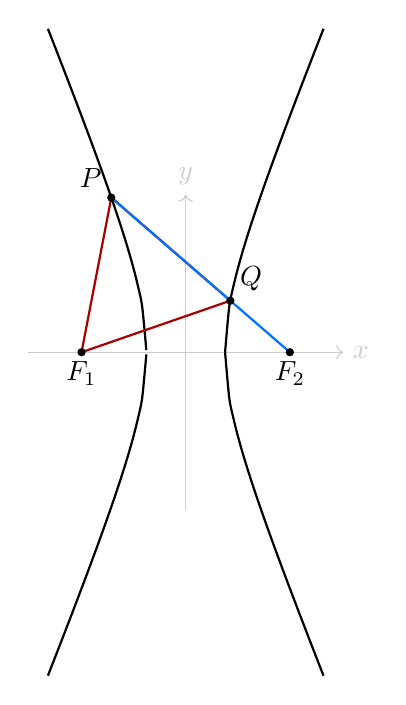
\begin{tikzpicture}[scale=0.5, baseline=(current bounding box.north)]
		\pgfmathsetmacro{\a}{1}
		\pgfmathsetmacro{\c}{sqrt(7)}
		\pgfmathsetmacro{\b}{sqrt(6)}
		
		\draw[->, gray!40] (-4,0) -- (4,0) node[right] {$x$};
		\draw[->, gray!40] (0,-4) -- (0,4) node[above] {$y$};
		
		% 双曲线 x^2 - y^2/6 = 1
		\draw[thick, domain=1:3.5, smooth, variable=\x] plot ({\x}, {\b*sqrt(\x*\x-1)/\a});
		\draw[thick, domain=1:3.5, smooth, variable=\x] plot ({\x}, {-\b*sqrt(\x*\x-1)/\a});
		\draw[thick, domain=-3.5:-1, smooth, variable=\x] plot ({\x}, {\b*sqrt(\x*\x-1)/\a});
		\draw[thick, domain=-3.5:-1, smooth, variable=\x] plot ({\x}, {-\b*sqrt(\x*\x-1)/\a});
		
		\coordinate (F1) at (-\c, 0);
		\coordinate (F2) at (\c, 0);
		\coordinate (P) at ({-5/\c}, {sqrt(108/7)});
		\coordinate (Q) at ({3/\c}, {sqrt(12/7)});
		
		\draw[thick, DarkRed] (P) -- (F1) -- (Q) -- cycle;
		\draw[thick, SkyBlue] (P) -- (F2);
		
		\fill (F1) circle (3pt) node[below] {$F_1$};
		\fill (F2) circle (3pt) node[below] {$F_2$};
		\fill (P) circle (3pt) node[above left] {$P$};
		\fill (Q) circle (3pt) node[above right] {$Q$};
	\end{tikzpicture}
\end{minipage}

\subsection{第七讲\quad 抛物线初步}

\subsubsection{定义}
\begin{knowledge}{抛物线的定义}
	平面内与一个定点 $F$ 和一条定直线 $l$ ($l$ 不经过 $F$) 的距离相等的点的轨迹叫抛物线.
	\begin{itemize}
		\item 定点 $F$：焦点.
		\item 定直线 $l$：准线.
		\item $F$ 与 $l$ 的距离为焦准距 $p$ ($p>0$).
	\end{itemize}
	\textbf{注意：}若 $F$ 在 $l$ 上，轨迹为过 $F$ 且垂直于 $l$ 的直线.
\end{knowledge}

\category{圆锥曲线定义对比}
\begin{enumerate}[label=\arabic*.]
	\item 一个定点：圆（到定点距离为定值）.
	\item 两个定点（对称）：
	\begin{itemize}
		\item 椭圆：$|PF_1|+|PF_2|=2a$ ($2a > |F_1F_2|$)
		\item 双曲线：$||PF_1|-|PF_2||=2a$ ($2a < |F_1F_2|$)
	\end{itemize}
	\item 一个直线 + 一个点：直线或抛物线.
\end{enumerate}

\subsubsection{标准方程}
\begin{knowledge}{标准方程形式}
	$y^2=2px$ ($p>0$).
	\begin{itemize}
		\item \textbf{判断焦点位置：}谁是一次项，焦点在谁上（$x$ 或 $y$ 轴）.
		\item \textbf{判断开口方向：}系数正，开口向正半轴；系数负，开口向负半轴.
		\item \textbf{焦点坐标：}一次项变量轴上，坐标值为 $\frac{1}{4} \times$ 一次项系数（即 $\frac{p}{2}$）.
	\end{itemize}
\end{knowledge}

\begin{question}
	已知抛物线 $y=\frac{1}{2}x^2$，求准线方程.
\end{question}

化为标准方程：$x^2=2y$.
焦点在 $y$ 轴，$2p=2 \implies p=1$.
焦点 $(0, \frac{1}{2})$，准线 $y=-\frac{1}{2}$.

\begin{question}
	求过点 $(1,2)$ 的抛物线方程.
\end{question}

\begin{minipage}[t]{0.7\textwidth}
	需分类讨论开口方向：
	\begin{enumerate}[label=\arabic*.]
		\item 开口向上（焦点在 $y$ 轴）：设 $x^2=2py$.
		代入 $(1,2) \implies 1=4p \implies 2p=\frac{1}{2}$.
		方程：$x^2=\frac{1}{2}y$.
		\item 开口向右（焦点在 $x$ 轴）：设 $y^2=2px$.
		代入 $(1,2) \implies 4=2p$.
		方程：$y^2=4x$.
	\end{enumerate}
\end{minipage}
\hfill
\begin{minipage}[t]{0.3\textwidth}
	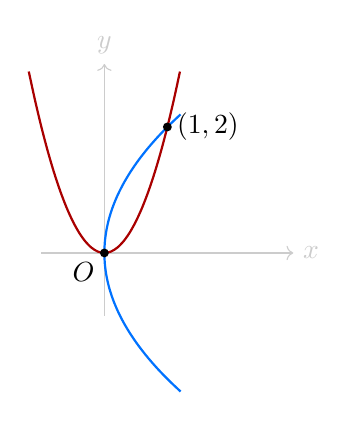
\begin{tikzpicture}[scale=0.8, baseline=(current bounding box.north)]
		\draw[->, gray!40] (-1,0) -- (3,0) node[right] {$x$};
		\draw[->, gray!40] (0,-1) -- (0,3) node[above] {$y$};
		% x^2 = 0.5y => y = 2x^2
		\draw[thick, DarkRed, domain=-1.2:1.2, smooth, variable=\x] plot ({\x}, {2*\x*\x});
		% y^2 = 4x => x = 0.25y^2
		\draw[thick, SkyBlue, domain=-2.2:2.2, smooth, variable=\y] plot ({0.25*\y*\y}, {\y});
		
		\fill (1,2) circle (2pt) node[right] {$(1,2)$};
		\fill (0,0) circle (2pt) node[below left] {$O$};
	\end{tikzpicture}
\end{minipage}

\subsubsection{定义与焦准距转化}
\begin{question}
	若焦准距为 2，求抛物线方程.
\end{question}

$p=2$.抛物线有四种开口方向：
\[
\begin{cases}
	x^2 = \pm 2py = \pm 4y \\
	y^2 = \pm 2px = \pm 4x
\end{cases}
\]

\begin{knowledge}{焦半径公式（定义转化）}
	设 $P(x_0, y_0)$ 为抛物线 $y^2=2px$ 上一点.
	
	$|PF| = |P\text{到准线}| = x_0 + \frac{p}{2}$.
	
	\textbf{用途：}涉及抛物线上一点到焦点的距离，常转化为到准线的距离.
\end{knowledge}

\begin{minipage}[t]{0.7\textwidth}
	
	
	\textbf{示例：}
	对于 $y^2=2px$，准线 $x=-\frac{p}{2}$.
	
	$|PF| = x_0 - (-\frac{p}{2}) = x_0 + \frac{p}{2}$.
	
	对于 $x^2=2py$，准线 $y=-\frac{p}{2}$.
	$|PF| = y_0 - (-\frac{p}{2}) = y_0 + \frac{p}{2}$.
\end{minipage}
\hfill
\begin{minipage}[t]{0.3\textwidth}
	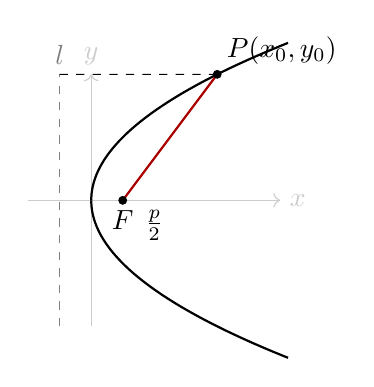
\begin{tikzpicture}[scale=0.8, baseline=(current bounding box.north)]
		\draw[->, gray!40] (-1,0) -- (3,0) node[right] {$x$};
		\draw[->, gray!40] (0,-2) -- (0,2) node[above] {$y$};
		% y^2 = 2x (p=1)
		\draw[thick, domain=0:2.5, smooth, variable=\y] plot ({0.5*\y*\y}, {\y});
		\draw[thick, domain=0:2.5, smooth, variable=\y] plot ({0.5*\y*\y}, {-\y});
		
		\coordinate (F) at (0.5, 0);
		\coordinate (P) at (2, 2); % 2^2 = 2*2 no, 4=4. y^2=2x -> 4=2*2. P(2,2) is on y^2=2x? 4=4 yes.
		% Wait, y^2=2px. If p=1, y^2=2x. P(2,2) -> 4=4. Correct.
		% Focus (0.5, 0). Directrix x = -0.5.
		
		\draw[dashed, gray] (-0.5,-2) -- (-0.5,2) node[above] {$l$};
		\draw[dashed] (P) -- (-0.5, 2); % Perpendicular to directrix
		\draw[thick, DarkRed] (P) -- (F);
		
		\fill (F) circle (2pt) node[below] {$F$};
		\fill (P) circle (2pt) node[above right] {$P(x_0,y_0)$};
		\node[below] at (1, 0) {$\frac{p}{2}$};
	\end{tikzpicture}
\end{minipage}

\subsubsection{将军饮马问题}
	\begin{minipage}{0.5\textwidth}
		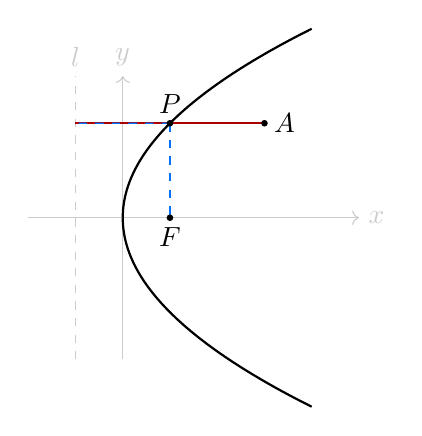
\begin{tikzpicture}[scale=0.6, baseline=(current bounding box.north)]
			\draw[->, gray!40] (-2,0) -- (5,0) node[right] {$x$};
			\draw[->, gray!40] (0,-3) -- (0,3) node[above] {$y$};
			\draw[dashed, gray!40] (-1,-3) -- (-1,3) node[above] {$l$};
			
			% 抛物线 y^2=4x
			\draw[thick, domain=0:4, smooth, variable=\y] plot ({0.25*\y*\y}, {\y});
			\draw[thick, domain=0:4, smooth, variable=\y] plot ({0.25*\y*\y}, {-\y});
			
			\coordinate (F) at (1,0);
			\coordinate (A) at (3,2);
			\coordinate (P) at (1,2);
			\coordinate (Aproj) at (-1,2);
			
			% 最短路径：A到准线的垂线
			\draw[thick, DarkRed] (A) -- (Aproj);
			% 转化：|PF| = d
			\draw[dashed, SkyBlue] (P) -- (F);
			\draw[dashed, SkyBlue] (P) -- (-1,2);
			
			\fill[black] (F) circle (2pt) node[below] {$F$};
			\fill[black] (A) circle (2pt) node[right] {$A$};
			\fill[black] (P) circle (2pt) node[above] {$P$};
		\end{tikzpicture}
		
		$AP+PF=x_A+\dfrac{p}{2}$
	\end{minipage}
	\hfill
	\begin{minipage}{0.5\textwidth}
		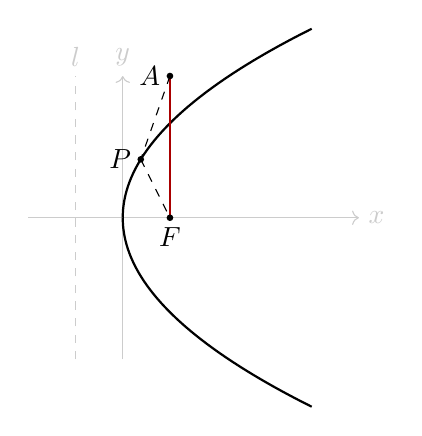
\begin{tikzpicture}[scale=0.6, baseline=(current bounding box.north)]
			\draw[->, gray!40] (-2,0) -- (5,0) node[right] {$x$};
			\draw[->, gray!40] (0,-3) -- (0,3) node[above] {$y$};
			\draw[dashed, gray!40] (-1,-3) -- (-1,3) node[above] {$l$};
			
			% 抛物线 y^2=4x
			\draw[thick, domain=0:4, smooth, variable=\y] plot ({0.25*\y*\y}, {\y});
			\draw[thick, domain=0:4, smooth, variable=\y] plot ({0.25*\y*\y}, {-\y});
			
			\pgfmathsetmacro{\px}{(3-sqrt(5))/2}
			\pgfmathsetmacro{\py}{sqrt(5)-1}
			
			\coordinate (F) at (1,0);
			\coordinate (A) at (1,3);
			\coordinate (P) at (\px, \py);
			
			% 最短路径：|AF|
			\draw[thick, DarkRed] (A) -- (F);
			% 转化：d = |PF|
%			\draw[dashed, SkyBlue] (P) -- (-1, \py);
%			\draw[dashed, SkyBlue] (P) -- (F);
			
			\fill[black] (F) circle (2pt) node[below] {$F$};
			\fill[black] (A) circle (2pt) node[left] {$A$};
			\fill[black] (P) circle (2pt) node[left] {$P$};
			\draw[dashed,black] (A)--(P);
			\draw[dashed,black] (P)--(F);
		\end{tikzpicture}
		
		$(AP+PF)_\text{min}=AF$
	\end{minipage}

\category{将军饮马问题（定义转化）}
\begin{question}
	已知抛物线$y^2=2px$经过点$M(x_0, 2\sqrt{2})$，若$M$到准线$l$距离为$3$，求方程.
\end{question}

$M$到$l$距离$= x_0 + \dfrac{p}{2} = 3$.

将$M$代入抛物线方程：$(2\sqrt{2})^2 = 2px_0 \implies 8 = 2px_0 \implies x_0 = \dfrac{4}{p}$.

$\dfrac{p}{2} + \dfrac{4}{p} = 3 \implies p^2 - 6p + 8 = 0 \implies p=4$或$p=2$.

$\therefore$方程为$y^2=4x$或$y^2=8x$.

\subsubsection{相似三角形问题}
\begin{knowledge}{梯形中位线推广}
	如图，直角梯形上底为$a$，下底为$b$.
	
	若中间平行线$c$将腰分为$1:3$（上段:下段），则：
	\[
	c = \frac{3}{4}a + \frac{1}{4}b
	\]
	\textbf{应用：}在抛物线焦点弦问题中，若$\overrightarrow{AF}=\lambda\overrightarrow{FB}$，则焦准距$p$满足定比分点关系.
\end{knowledge}

\begin{minipage}[t]{0.7\textwidth}
	\textbf{推导：}
	设上底$a$，下底$b$，高$h$.
	腰被分为$1:3$，则$c$距离上底$\frac{1}{4}h$.
	由相似三角形或线性插值：
	\[
	c = a + \frac{1}{4}(b-a) = \frac{3}{4}a + \frac{1}{4}b
	\]
\end{minipage}
\hfill
\begin{minipage}[t]{0.3\textwidth}
	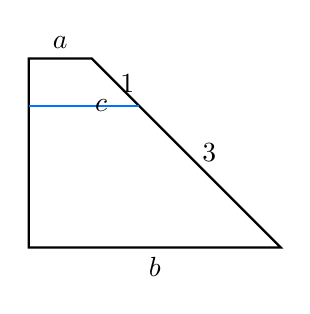
\begin{tikzpicture}[scale=0.8, baseline=(current bounding box.north)]
		\coordinate (A) at (0, 3);
		\coordinate (B) at (1, 3);
		\coordinate (C) at (4, 0);
		\coordinate (D) at (0, 0);
		\coordinate (P) at (1.75, 2.25);
		\coordinate (Q) at (0, 2.25);
		
		\draw[thick] (D) -- (C) -- (B) -- (A) -- cycle;
		\draw[thick, SkyBlue] (Q) -- (P);
		
		\node[above] at (0.5, 3) {$a$};
		\node[below] at (2, 0) {$b$};
		\node[right] at (0.9, 2.25) {$c$};
		
		\node[right] at (1.3, 2.6) {$1$};
		\node[right] at (2.6, 1.5) {$3$};
	\end{tikzpicture}
\end{minipage}

\category{相似三角形问题（最值）}
\begin{question}
	已知$y^2=4x$，$A(5,3)$，$M$为抛物线上一点，求$\triangle MAF$周长最小值.
\end{question}

\begin{minipage}[t]{0.7\textwidth}
	$F(1,0)$，准线$l: x=-1$.
	
	$|AF| = \sqrt{(5-1)^2 + 3^2} = 5$（定值）.
	
	周长$C = |MA| + |MF| + |AF| = |MA| + d(M, l) + 5$.
	
	当$M, A$与$M$在准线上的投影$M'$三点共线（即$MA \perp l$）时，
	
	$|MA| + d(M, l)$最小.
	
	最小值$= d(A, l) = 5 - (-1) = 6$.
	
	$\therefore C_{\min} = 6 + 5 = 11$.
\end{minipage}
\hfill
\begin{minipage}[t]{0.3\textwidth}
	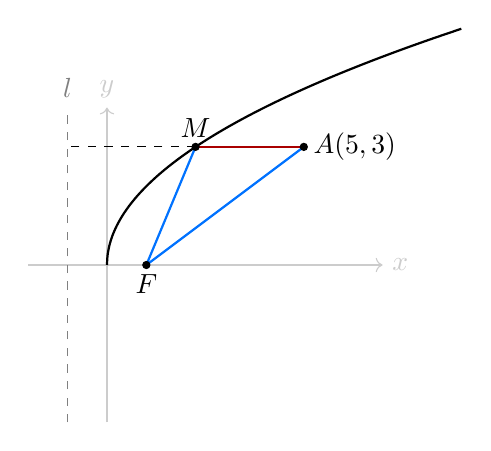
\begin{tikzpicture}[scale=0.5, baseline=(current bounding box.north)]
		\draw[->, gray!40] (-2,0) -- (7,0) node[right] {$x$};
		\draw[->, gray!40] (0,-4) -- (0,4) node[above] {$y$};
		\draw[dashed, gray] (-1,-4) -- (-1,4) node[above] {$l$};
		% y^2=4x
		\draw[thick, domain=0:6, smooth, variable=\y] plot ({0.25*\y*\y}, {\y});
		
		\coordinate (F) at (1,0);
		\coordinate (A) at (5,3);
		\coordinate (M) at (2.25, 3); % y=3, x=9/4=2.25
		
		\draw[thick, DarkRed] (A) -- (M);
		\draw[thick, SkyBlue] (M) -- (F);
		\draw[thick, SkyBlue] (A) -- (F);
		\draw[dashed] (M) -- (-1, 3);
		
		\fill (F) circle (3pt) node[below] {$F$};
		\fill (A) circle (3pt) node[right] {$A(5,3)$};
		\fill (M) circle (3pt) node[above] {$M$};
	\end{tikzpicture}
\end{minipage}

\begin{question}
	$P$在抛物线$y^2=4x$上，则$P$到$A(0,-1)$的距离与到直线$x=-1$的距离之和的最小值.
\end{question}

\begin{minipage}[t]{0.7\textwidth}
	$P$到直线$x=-1$（准线）的距离等于$|PF|$（$F$为焦点$(1,0)$）.
	
	即求$|PA| + |PF|$的最小值.
	
	$\because$ 线段$AF$与抛物线相交.
	
	$\therefore$ 最小值$= |AF| = \sqrt{(1-0)^2 + (0-(-1))^2} = \sqrt{2}$.
\end{minipage}
\hfill
\begin{minipage}[t]{0.3\textwidth}
	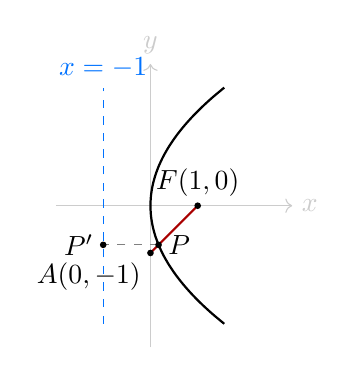
\begin{tikzpicture}[scale=0.6, baseline=(current bounding box.north)]
		\draw[->, gray!40] (-2,0) -- (3,0) node[right] {$x$};
		\draw[->, gray!40] (0,-3) -- (0,3) node[above] {$y$};
		
		% 抛物线 y^2=4x
		\draw[thick, domain=-2.5:2.5, smooth, variable=\y] plot ({0.25*\y*\y}, {\y});
		
		% 准线 x=-1
		\draw[dashed, SkyBlue] (-1,-2.5) -- (-1,2.5) node[above] {$x=-1$};
		
		% 坐标点
		\coordinate (A) at (0,-1);
		\coordinate (F) at (1,0);
		\coordinate (P) at ({3-2*sqrt(2)}, {2-2*sqrt(2)});
		\coordinate (P_proj) at (-1, {2-2*sqrt(2)});
		
		% 连线
		\draw[thick, DarkRed] (A) -- (F);
		\draw[dashed, gray] (P) -- (P_proj);
		
		% 标点
		\fill (A) circle (2pt) node[below left] {$A(0,-1)$};
		\fill (F) circle (2pt) node[above] {$F(1,0)$};
		\fill (P) circle (2pt) node[right] {$P$};
		\fill (P_proj) circle (2pt) node[left] {$P'$};
	\end{tikzpicture}
\end{minipage}

\category{焦点弦与向量}
\begin{question}
	已知$y^2=4x$，$A,B$在抛物线上，$\overrightarrow{AF}=3\overrightarrow{FB}$，则$|AB|=$?
\end{question}

\begin{minipage}[t]{0.7\textwidth}
	$p=2$，焦点$F(1,0)$，准线$x=-1$.
	
	设$|BF|=x$，则$|AF|=3x$，$|AB|=4x$.
	
	由梯形中位线推广（或相似三角形）：
	$F$到准线距离$p=2$.
	
	$A, B$到准线距离分别为$|AF|=3x, |BF|=x$.
	
	$F$分$AB$为$3:1$，则$p = \dfrac{1 \cdot |AF| + 3 \cdot |BF|}{1+3}$（定比分点公式）.
	
	$2 = \dfrac{3x + 3x}{4} = \dfrac{6x}{4} = \dfrac{3}{2}x$.
	
	$\therefore x = \dfrac{4}{3}$.
	
	$\therefore |AB| = 4x = \dfrac{16}{3}$.
\end{minipage}
\hfill
\begin{minipage}[t]{0.3\textwidth}
	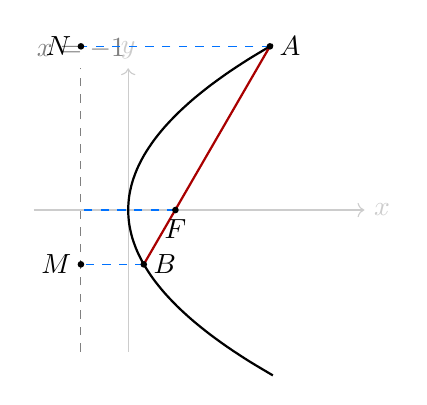
\begin{tikzpicture}[scale=0.6, baseline=(current bounding box.north)]
		\draw[->, gray!40] (-2,0) -- (5,0) node[right] {$x$};
		\draw[->, gray!40] (0,-3) -- (0,3) node[above] {$y$};
		\draw[dashed, gray] (-1,-3) -- (-1,3) node[above] {$x=-1$};
		% y^2=4x
		\draw[thick, domain=-3.5:3.5, smooth, variable=\y] plot ({0.25*\y*\y}, {\y});
		
		\coordinate (F) at (1,0);
		\coordinate (A) at (3, {2*sqrt(3)}); % approx (3, 3.46)
		\coordinate (B) at (0.33, {-1.15}); % approx (1/3, -2sqrt(3)/3)
		\coordinate (N) at (-1, {2*sqrt(3)});
		\coordinate (M) at (-1, {-1.15});
		
		\draw[thick, DarkRed] (A) -- (B);
		\draw[dashed, SkyBlue] (A) -- (N);
		\draw[dashed, SkyBlue] (B) -- (M);
		\draw[dashed, SkyBlue] (F) -- (-1, 0);
		
		\fill (F) circle (2pt) node[below] {$F$};
		\fill (A) circle (2pt) node[right] {$A$};
		\fill (B) circle (2pt) node[right] {$B$};
		\fill (N) circle (2pt) node[left] {$N$};
		\fill (M) circle (2pt) node[left] {$M$};
	\end{tikzpicture}
\end{minipage}

\subsection{第八讲\quad 轨迹方程}

\subsubsection{圆锥曲线综合(求方程/离心率)}

\begin{knowledge}{}
	求方程：
	
	双曲线/椭圆：焦点+ 2条件
	
	抛物线：焦点位置$\Bigg\{(\pm \dfrac{p}{2},0) ~\text{or}~ (0,\pm \dfrac{p}{2})\Bigg\}$+ 1条件 求p
\end{knowledge}


\category{圆锥曲线综合}
\begin{question}
	双曲线$C_1:\dfrac{x^2}{a^2}-\dfrac{y^2}{b^2}=1\ (e=2)$，抛物线$C_2:x^2=2py\ (p>0)$的焦点到双曲线$C_1$的渐近线的距离为$2$，求抛物线方程.
\end{question}

抛物线焦点坐标为$(0, \dfrac{p}{2})$.

由双曲线离心率$e=\sqrt{1+\dfrac{b^2}{a^2}}=2 \implies \dfrac{b}{a}=\sqrt{3}$.

渐近线方程为$y=\pm\sqrt{3}x \implies \sqrt{3}x-y=0$.

由点到直线距离公式：
\[
d = \frac{|\sqrt{3}\cdot 0 - \frac{p}{2}|}{\sqrt{(\sqrt{3})^2+(-1)^2}} = \dfrac{\frac{p}{2}}{2} = 2 \implies p=8.
\]

$\therefore$ 抛物线方程为$x^2=16y$.

\category{轨迹方程（面积法）}
\begin{question}
	已知椭圆$\dfrac{x^2}{a^2}+\dfrac{y^2}{b^2}=1$的$e=\dfrac{\sqrt{2}}{2}$，双曲线$x^2-y^2=1$的渐近线与椭圆有$4$个交点，$4$交点围成的四边形$S=16$，求椭圆方程.
\end{question}

\begin{minipage}[t]{0.7\textwidth}
	双曲线$x^2-y^2=1$的渐近线为$y=\pm x$（倾斜角$45^\circ$）.
	
	由椭圆离心率$e=\dfrac{c}{a}=\dfrac{\sqrt{2}}{2} \implies a^2=2b^2$.
	
	渐近线$y=\pm x$与坐标轴夹角$45^\circ$，围成的四边形为正方形（对角线在$y=\pm x$上）.
	
	$\because S=16$，由对称性，第一象限交点为$(2,2)$.
	
	将$a^2=2b^2$及点$(2,2)$代入椭圆方程：
	\[
	\frac{4}{2b^2} + \frac{4}{b^2} = 1 \implies \frac{2}{b^2} + \frac{4}{b^2} = 1 \implies b^2=6.
	\]
	$\therefore a^2=12$.
	
	椭圆方程为$\dfrac{x^2}{12}+\dfrac{y^2}{6}=1$.
\end{minipage}
\hfill
\begin{minipage}[t]{0.3\textwidth}
	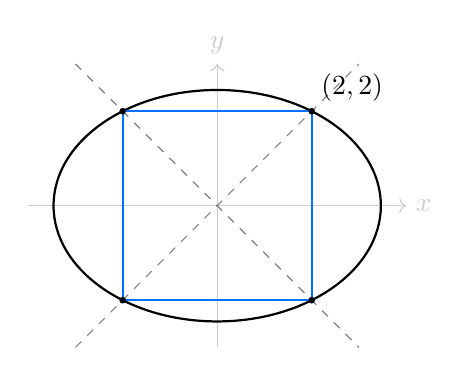
\begin{tikzpicture}[scale=0.6, baseline=(current bounding box.north)]
		\draw[->, gray!40] (-4,0) -- (4,0) node[right] {$x$};
		\draw[->, gray!40] (0,-3) -- (0,3) node[above] {$y$};
		
		% 椭圆 x^2/12 + y^2/6 = 1 -> a=sqrt(12)~3.46, b=sqrt(6)~2.45
		\draw[thick] (0,0) ellipse ({sqrt(12)} and {sqrt(6)});
		
		% 渐近线 y=x, y=-x
		\draw[dashed, gray] (-3,-3) -- (3,3);
		\draw[dashed, gray] (-3,3) -- (3,-3);
		
		% 交点 (2,2), (-2,2), (-2,-2), (2,-2)
		\coordinate (P1) at (2,2);
		\coordinate (P2) at (-2,2);
		\coordinate (P3) at (-2,-2);
		\coordinate (P4) at (2,-2);
		
		\draw[thick, SkyBlue] (P1) -- (P2) -- (P3) -- (P4) -- cycle;
		
		\fill (P1) circle (2pt) node[above right] {$(2,2)$};
		\fill (P2) circle (2pt);
		\fill (P3) circle (2pt);
		\fill (P4) circle (2pt);
	\end{tikzpicture}
\end{minipage}

\category{共焦点问题}
\begin{question}
	如图，$F_1,F_2$为椭圆$\dfrac{x^2}{4}+y^2=1$与双曲线的共焦点. 若$AF_1BF_2$为矩形，求双曲线的离心率.
\end{question}

\begin{minipage}[t]{0.7\textwidth}
	椭圆中$a_1^2=4, b_1^2=1 \implies c^2=3 \implies c=\sqrt{3}$.
	
	双曲线与椭圆共焦点，故双曲线$c=\sqrt{3}$.
	
	$\because$ 四边形$AF_1BF_2$为矩形
	
	$\therefore$ 对角线相等且互相平分.
	
	$\therefore |OA|=|OF_1|=c$.
	
	$\therefore \triangle F_1AF_2$为直角三角形，$\angle F_1AF_2=90^\circ$.
	
	由椭圆定义：$|AF_1|+|AF_2|=2a_1=4$.
	
	由勾股定理：$|AF_1|^2+|AF_2|^2=|F_1F_2|^2=(2c)^2=12$.
	
	联立解得：$2|AF_1||AF_2| = (|AF_1|+|AF_2|)^2 - (|AF_1|^2+|AF_2|^2) = 16-12=4$.
	
	由双曲线定义：$2a_2 = ||AF_2|-|AF_1||$.
	
	$(2a_2)^2 = (|AF_2|-|AF_1|)^2 = |AF_1|^2+|AF_2|^2 - 2|AF_1||AF_2| = 12-4=8$.
	
	$\therefore 4a_2^2=8 \implies a_2=\sqrt{2}$.
	
	$\therefore$ 双曲线离心率$e_2 = \dfrac{c}{a_2} = \dfrac{\sqrt{3}}{\sqrt{2}} = \dfrac{\sqrt{6}}{2}$.
\end{minipage}
\hfill
\begin{minipage}[t]{0.3\textwidth}
	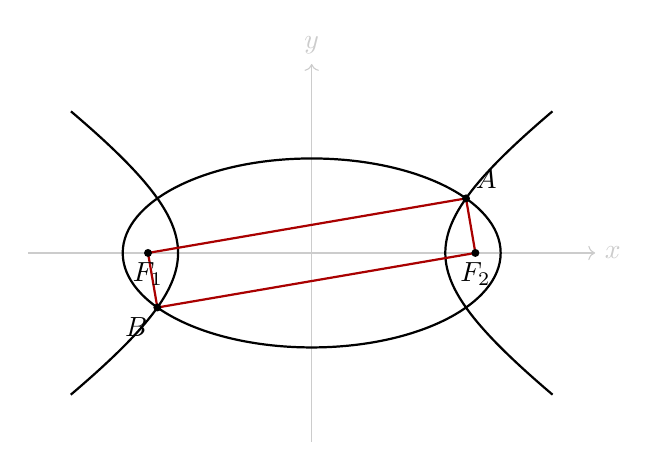
\begin{tikzpicture}[scale=1.2, baseline=(current bounding box.north)]
		\draw[->, gray!40] (-3,0) -- (3,0) node[right] {$x$};
		\draw[->, gray!40] (0,-2) -- (0,2) node[above] {$y$};
		
		% 椭圆 x^2/4 + y^2 = 1
		\draw[thick] (0,0) ellipse (2 and 1);
		
		% 双曲线 x^2/2 - y^2 = 1，使用y作自变量避免断点和负数开方
		\draw[thick, domain=-1.5:1.5, smooth, samples=100, variable=\y] plot ({sqrt(2*(\y*\y+1))}, {\y});
		\draw[thick, domain=-1.5:1.5, smooth, samples=100, variable=\y] plot ({-sqrt(2*(\y*\y+1))}, {\y});
		
		\coordinate (F1) at ({-sqrt(3)}, 0);
		\coordinate (F2) at ({sqrt(3)}, 0);
		\coordinate (A) at ({sqrt(8/3)}, {sqrt(1/3)});
		\coordinate (B) at ({-sqrt(8/3)}, {-sqrt(1/3)});
		
		\draw[thick, DarkRed] (A) -- (F1) -- (B) -- (F2) -- cycle;
		
		\fill (F1) circle (1.2pt) node[below] {$F_1$};
		\fill (F2) circle (1.2pt) node[below] {$F_2$};
		\fill (A) circle (1.2pt) node[above right] {$A$};
		\fill (B) circle (1.2pt) node[below left] {$B$};
	\end{tikzpicture}
\end{minipage}

\subsection*{2. 轨迹方程}

\begin{knowledge}{直接法}
	翻动条件形成数字表达式.
	
	注意分母不为0，$\triangle ABC$ (不共线).
\end{knowledge}

\begin{question}
	自圆 $(x-3)^2+(y+4)^2=4$ 外一点 $P(x,y)$ 引一条切线，切线长 $=OP$，求 $P$ 的轨迹方程.
\end{question}

\begin{minipage}[t]{0.7\textwidth}
	圆心 $C(3,-4)$，半径 $r=2$.
	
	切线长 $PQ = \sqrt{PC^2-r^2} = \sqrt{(x-3)^2+(y+4)^2-4}$.
	
	$OP = \sqrt{x^2+y^2}$.
	
	由题意 $PQ=OP \implies PQ^2=OP^2$.
	
	$(x-3)^2+(y+4)^2-4 = x^2+y^2$.
	
	$x^2-6x+9+y^2+8y+16-4 = x^2+y^2$.
	
	$-6x+8y+21=0$.
	
	$\therefore 6x-8y-21=0$.
\end{minipage}
\hfill
\begin{minipage}[t]{0.3\textwidth}
	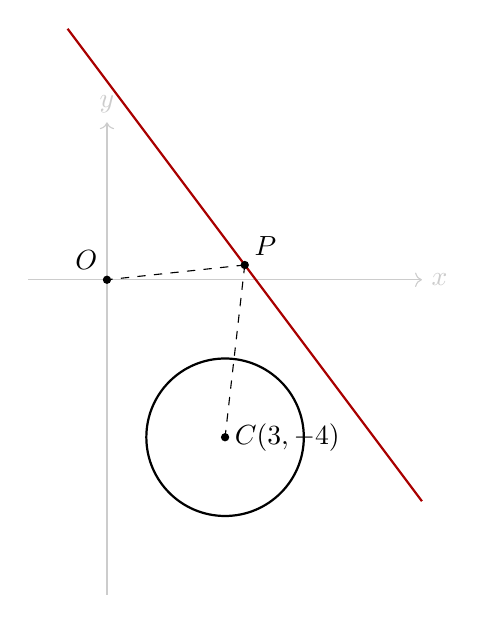
\begin{tikzpicture}[scale=0.5, baseline=(current bounding box.north)]
		\draw[->, gray!40] (-2,0) -- (8,0) node[right] {$x$};
		\draw[->, gray!40] (0,-8) -- (0,4) node[above] {$y$};
		
		\coordinate (C) at (3,-4);
		\coordinate (O) at (0,0);
		\coordinate (P) at (3.5, 0.375); % 6(3.5)-8(0.375)-21 = 21-3-21=-3 approx 0
		
		\draw[thick] (C) circle (2);
		\draw[thick, DarkRed] (-1, 6.375) -- (8, -5.625); % 6x-8y-21=0 -> y = 0.75x - 2.625
		
		\draw[dashed] (P) -- (C);
		\draw[dashed] (P) -- (O);
		
		\fill (C) circle (3pt) node[right] {$C(3,-4)$};
		\fill (O) circle (3pt) node[above left] {$O$};
		\fill (P) circle (3pt) node[above right] {$P$};
	\end{tikzpicture}
\end{minipage}

\category{定义法}
\begin{knowledge}{曲线类型判断}
	根据 $mx^2+ny^2=1$:
	\begin{enumerate}
		\item $m=n>0$ 圆.
		
		\item $m \neq n > 0$ 椭圆.
		
		\item $m \cdot n < 0$ 双曲线.
		
		\item $m, n < 0$ 不存在.
	\end{enumerate}
	
	\textbf{猜哪种曲线步骤：}
	\begin{enumerate}
		\item 一点：圆.
		
		\item 两点：椭圆 ($|PF_1|+|PF_2|=2a, a>c$)，双曲线 ($||PF_1|-|PF_2||=2a, c>a$) $\implies$ 双曲线一支 (有范围).
		
		\item 一点一线：抛物线.
	\end{enumerate}
\end{knowledge}



\category{相关点法}
\begin{knowledge}{相关点法步骤}
	\begin{enumerate}
		\item 设轨迹点 $(x,y)$，相关点 $(x_0,y_0)$.
		
		\item 用 $x,y$ 表示 $x_0,y_0$.
		
		\item 分离 $x_0,y_0$.
		
		\item 把 $x_0,y_0$ 代入相关表达式中.
	\end{enumerate}
\end{knowledge}

\begin{question}
	$P$ 是 $x^2+y^2+4x-12y+39=0$ 上的动点，直线 $x-y+1=0$ 是 $PQ$ 中垂线，求 $Q$ 的轨迹方程.
\end{question}

\begin{minipage}[t]{0.7\textwidth}
	圆方程：$(x+2)^2+(y-6)^2=1$，圆心 $C(-2,6)$，半径 $r=1$.
	
	设 $Q(x,y), P(x_0,y_0)$.
	
	$PQ \perp l$ 且中点在 $l$ 上.
	
	$\begin{cases} \frac{y-y_0}{x-x_0} = -1 \\ \frac{x_0+x}{2} - \frac{y_0+y}{2} + 1 = 0 \end{cases} \implies \begin{cases} x_0 = y-1 \\ y_0 = x+1 \end{cases}$
	
	代入圆方程 $(x_0+2)^2+(y_0-6)^2=1$:
	
	$(y-1+2)^2 + (x+1-6)^2 = 1$.
	
	$\therefore (x-5)^2 + (y+1)^2 = 1$.
\end{minipage}
\hfill
\begin{minipage}[t]{0.3\textwidth}
	\begin{tikzpicture}[scale=0.5, baseline=(current bounding box.north)]
		\draw[->, gray!40] (-6,0) -- (6,0) node[right] {$x$};
		\draw[->, gray!40] (0,-4) -- (0,10) node[above] {$y$};
		
		\coordinate (C) at (-2,6);
		\coordinate (P) at (-1.5, 6.866); % on circle
		\coordinate (Q) at (5.866, 0.5); % symmetric to P wrt x-y+1=0
		
		\draw[thick] (C) circle (1);
		\draw[thick, DarkRed] (-4, -3) -- (6, 7); % x-y+1=0 -> y=x+1
		\draw[dashed] (P) -- (Q);
		\draw[dashed, SkyBlue] (C) -- (P);
		
		\fill (C) circle (3pt) node[left] {$C$};
		\fill (P) circle (3pt) node[above] {$P$};
		\fill (Q) circle (3pt) node[right] {$Q$};
	\end{tikzpicture}
\end{minipage}

\begin{question}
	有一圆，圆心为 $O$，$Q$ 为圆外一点，$A$ 为圆上一点，使圆折叠后 $A$ 与 $Q$ 重合，折痕 $CD$ 与 $OA$ 交于 $P$，求 $P$ 的轨迹是什么图形.
\end{question}

\begin{minipage}[t]{0.7\textwidth}
	折叠 $\implies PA=PQ$.
	
	$P$ 在 $OA$ 直线上.
	
	$|PO - PQ| = |PO - PA| = OA = r$ (半径).
	
	$O, Q$ 是定点，$r$ 是常数.
	
	$\because Q$ 在圆外
	
	$\therefore OQ > r$.
	
	$\therefore |PO - PQ| = r < OQ$.
	
	$\therefore$ 轨迹为双曲线.
\end{minipage}
\hfill
\begin{minipage}[t]{0.3\textwidth}
	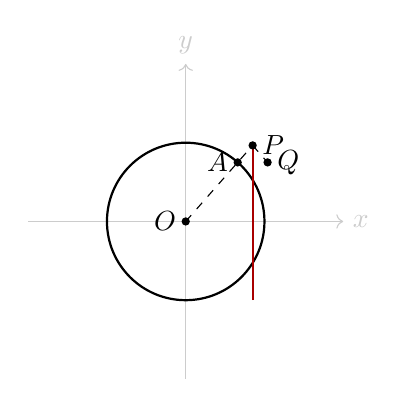
\begin{tikzpicture}[scale=0.5, baseline=(current bounding box.north)]
		\draw[->, gray!40] (-4,0) -- (4,0) node[right] {$x$};
		\draw[->, gray!40] (0,-4) -- (0,4) node[above] {$y$};
		
		\coordinate (O) at (0,0);
		\coordinate (Q) at (2.08,1.5);
		\coordinate (A) at (1.32, 1.5); % on circle r=2
		\coordinate (P) at (1.7, 1.931818); % on OA
		
		\draw[thick] (O) circle (2);
		\draw[thick, DarkRed] (1.7, -2) -- (1.7, 2); % Perpendicular bisector of AQ approx
		\draw[dashed] (O) -- (P);
		\draw[dashed] (P) -- (Q);
		
		\fill (O) circle (3pt) node[left] {$O$};
		\fill (Q) circle (3pt) node[right] {$Q$};
		\fill (A) circle (3pt) node[left] {$A$};
		\fill (P) circle (3pt) node[right] {$P$};
	\end{tikzpicture}
\end{minipage}

\category{动圆轨迹问题（定义法）}
\begin{question}
	动圆$M$与定圆$(x+2)^2+y^2=4$外切，且与直线$x=2$相切，求$M$的轨迹.
\end{question}

\begin{minipage}[t]{0.7\textwidth}
	定圆圆心$C(-2,0)$，半径$r=2$.
	
	设动圆$M$半径为$R$.
	由外切：$|MC| = R+2$.
	由与直线$x=2$相切：$M$到直线$x=2$的距离$d=R$.
	
	$\therefore \sqrt{(x+2)^2+y^2}-2=2-x$
	
	$\therefore y^2 = -12(x-1)$，即$y^2+12x-12=0$.
\end{minipage}
\hfill
\begin{minipage}[t]{0.3\textwidth}
	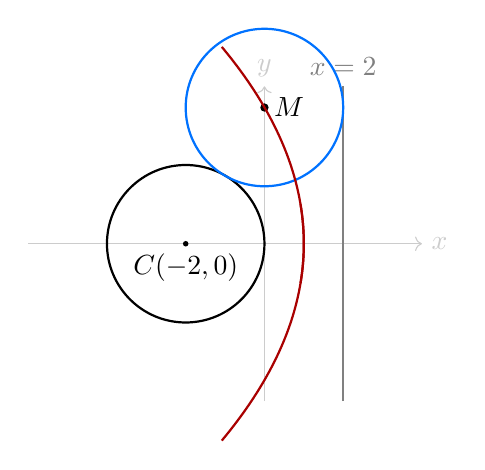
\begin{tikzpicture}[scale=0.5, baseline=(current bounding box.north)]
		\draw[->, gray!40] (-6,0) -- (4,0) node[right] {$x$};
		\draw[->, gray!40] (0,-4) -- (0,4) node[above] {$y$};
		
		% 定圆
		\draw[thick] (-2,0) circle (2);
		\fill (-2,0) circle (2pt) node[below] {$C(-2,0)$};
		
		% 直线 x=2
		\draw[thick, gray] (2,-4) -- (2,4) node[above] {$x=2$};
		
		% 动圆 M (示意)
		\coordinate (M) at (0, 2.45); % y^2 = -12(0-1) -> y=sqrt(12)~3.46. 取x=0, y=3.46. R=2.
		% 修正：取x=0, y^2=12, y=2sqrt(3)~3.46. R=2.
		% 距离C: sqrt(2^2 + 12) = 4. R+2 = 2+2=4. 对.
		\coordinate (M) at (0, 3.46);
		\draw[thick, SkyBlue] (M) circle (2);
		\fill (M) circle (3pt) node[right] {$M$};
		
		% 轨迹抛物线 y^2 = -12(x-1)
		\draw[thick, DarkRed, domain=-5:1, smooth, variable=\y] plot ({1-\y*\y/12}, {\y});
		\draw[thick, DarkRed, domain=-5:1, smooth, variable=\y] plot ({1-\y*\y/12}, {-\y});
		
	\end{tikzpicture}
\end{minipage}

\begin{question}
	动圆$P$与定圆$B:x^2+y^2+4x=0$相切，且过点$A(2,0)$，求$P$的轨迹.
\end{question}

定圆$B$：$(x+2)^2+y^2=4$，圆心$B(-2,0)$，半径$R=2$.

动圆$P$过点$A(2,0)$，设半径为$r$，则$|PA|=r$.

\textbf{情况1：外切}

$|PB| = R+r = 2+r$.

$|PB| - |PA| = 2$.

\textbf{情况2：内切}

$|PB| = |r-R| = |r-2|$.

若$P$包围$B$，则$r>2$，$|PB|=r-2$.

$|PA| - |PB| = r - (r-2) = 2$.


综上：$||PA|-|PB|| = 2$.

$\because |AB|=4 > 2$

$\therefore$ 轨迹为双曲线.

$2a=2 \implies a=1$. $2c=4 \implies c=2$.

$b^2 = c^2-a^2 = 3$.

方程：$x^2 - \dfrac{y^2}{3} = 1$.


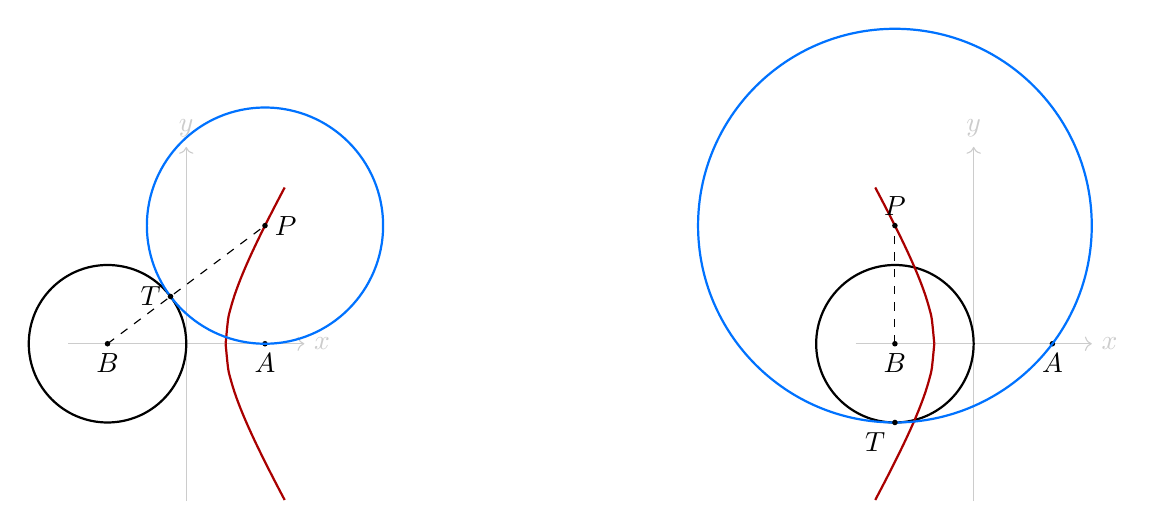
\begin{tikzpicture}[scale=0.5, baseline=(current bounding box.north)]
	% 左图：外切 (对应双曲线右支)
	\begin{scope}[shift={(-10,0)}]
		\draw[->, gray!40] (-3,0) -- (3,0) node[right] {$x$};
		\draw[->, gray!40] (0,-4) -- (0,5) node[above] {$y$};
		
		% 定圆 B
		\draw[thick] (-2,0) circle (2);
		\fill (-2,0) circle (2pt) node[below] {$B$};
		\fill (2,0) circle (2pt) node[below] {$A$};
		
		% 双曲线右支
		\draw[thick, DarkRed, domain=1:2.5, smooth, variable=\x] plot ({\x}, {sqrt(3*(\x*\x-1))});
		\draw[thick, DarkRed, domain=1:2.5, smooth, variable=\x] plot ({\x}, {-sqrt(3*(\x*\x-1))});
		
		% 动圆 P (圆心(2,3), 半径3)
		\coordinate (P) at (2,3);
		\draw[thick, SkyBlue] (P) circle (3);
		\fill (P) circle (2pt) node[right] {$P$};
		
		% 辅助线与切点 T(-0.4, 1.2)
		\draw[dashed] (-2,0) -- (2,3);
		\fill (-0.4, 1.2) circle (2pt) node[left] {$T$};
	\end{scope}
	
	% 右图：内切 (对应双曲线左支)
	\begin{scope}[shift={(10,0)}]
		\draw[->, gray!40] (-3,0) -- (3,0) node[right] {$x$};
		\draw[->, gray!40] (0,-4) -- (0,5) node[above] {$y$};
		
		% 定圆 B
		\draw[thick] (-2,0) circle (2);
		\fill (-2,0) circle (2pt) node[below] {$B$};
		\fill (2,0) circle (2pt) node[below] {$A$};
		
		% 双曲线左支
		\draw[thick, DarkRed, domain=-2.5:-1, smooth, variable=\x] plot ({\x}, {sqrt(3*(\x*\x-1))});
		\draw[thick, DarkRed, domain=-2.5:-1, smooth, variable=\x] plot ({\x}, {-sqrt(3*(\x*\x-1))});
		
		% 动圆 P (圆心(-2,3), 半径5)
		\coordinate (P) at (-2,3);
		\draw[thick, SkyBlue] (P) circle (5);
		\fill (P) circle (2pt) node[above] {$P$};
		
		% 辅助线与切点 T(-2, -2)
		\draw[dashed] (-2,0) -- (-2,3);
		\fill (-2,-2) circle (2pt) node[below left] {$T$};
	\end{scope}
\end{tikzpicture}

\category{根式方程求轨迹}
\begin{question}
	$M(x,y)$在运动时，满足$\sqrt{9+x^2+y^2+6y} - \sqrt{9+x^2-6y+y^2} = 4$，求$M$轨迹.
\end{question}

\begin{minipage}[t]{0.7\textwidth}
	化简根式：
	\[
	\sqrt{x^2+(y+3)^2} - \sqrt{x^2+(y-3)^2} = 4
	\]
	几何意义：$M$到点$F_1(0,-3)$的距离减去$M$到点$F_2(0,3)$的距离等于$4$.
	\[
	|MF_1| - |MF_2| = 4 = 2a
	\]
	$\because 2a=4 < |F_1F_2|=6$
	
	$\therefore$ 轨迹为双曲线的一支.
	
	焦点在$y$轴，$c=3, a=2$.
	
	$b^2 = c^2-a^2 = 9-4=5$.
	
	$\because |MF_1| > |MF_2|$，$M$离$F_2(0,3)$更近.
	
	$\therefore$ 轨迹为双曲线的上支.
	
	方程：$\dfrac{y^2}{4} - \dfrac{x^2}{5} = 1 \quad (y \ge 2)$.
\end{minipage}
\hfill
\begin{minipage}[t]{0.3\textwidth}
	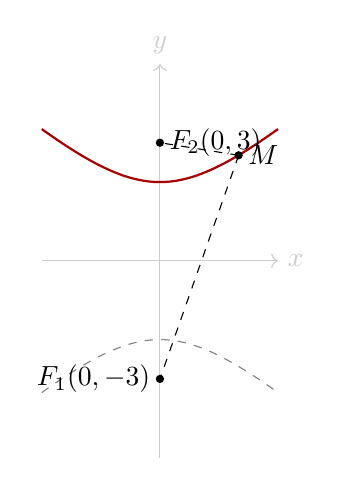
\begin{tikzpicture}[scale=0.5, baseline=(current bounding box.north)]
		\draw[->, gray!40] (-3,0) -- (3,0) node[right] {$x$};
		\draw[->, gray!40] (0,-5) -- (0,5) node[above] {$y$};
		
		% 双曲线 y^2/4 - x^2/5 = 1
		% y = 2*sqrt(1 + x^2/5)
		\draw[thick, DarkRed, domain=-3:3, smooth, variable=\x] plot ({\x}, {2*sqrt(1+\x*\x/5)});
		% 下支虚线
		\draw[dashed, gray, domain=-3:3, smooth, variable=\x] plot ({\x}, {-2*sqrt(1+\x*\x/5)});
		
		\fill (0,-3) circle (3pt) node[left] {$F_1(0,-3)$};
		\fill (0,3) circle (3pt) node[right] {$F_2(0,3)$};
		
		% 点 M
		\coordinate (M) at (2, 3.46); % x=2, y^2/4 - 4/5 = 1 -> y^2/4 = 1.8 -> y=sqrt(7.2)~2.68. 
		% 修正：取x=2. y = 2*sqrt(1+4/5) = 2*sqrt(1.8) ~ 2.68.
		\coordinate (M) at (2, 2.68);
		\fill (M) circle (3pt) node[right] {$M$};
		\draw[dashed] (M) -- (0,-3);
		\draw[dashed] (M) -- (0,3);
		
	\end{tikzpicture}
\end{minipage}

\category{动圆轨迹问题（定义法）}
\begin{question}
	动圆$P$与圆$A:(x+1)^2+y^2=1$外切，而与圆$B:(x-1)^2+y^2=9$内切，求$P$轨迹是什么图形.
\end{question}

\begin{minipage}[t]{0.7\textwidth}
	圆$A$：圆心$(-1,0)$，半径$r_A=1$.
	圆$B$：圆心$(1,0)$，半径$r_B=3$.
	
	设动圆$P$半径为$r$.
	由外切：$|PA| = r+1$.
	由内切（$P$在$B$内）：$|PB| = 3-r$.
	
	两式相加：
	\[
	|PA| + |PB| = (r+1) + (3-r) = 4.
	\]
	定点距离$|AB| = 2$.
	$\because 2a=4 > 2c=2$.
	$\therefore$ 轨迹为椭圆.
\end{minipage}
\hfill
\begin{minipage}[t]{0.3\textwidth}
	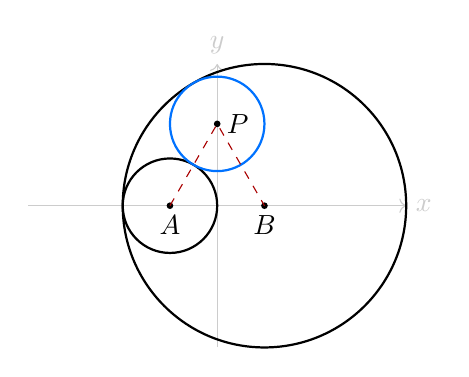
\begin{tikzpicture}[scale=0.6, baseline=(current bounding box.north)]
		\draw[->, gray!40] (-4,0) -- (4,0) node[right] {$x$};
		\draw[->, gray!40] (0,-3) -- (0,3) node[above] {$y$};
		
		% 圆 A
		\draw[thick] (-1,0) circle (1);
		\fill (-1,0) circle (2pt) node[below] {$A$};
		
		% 圆 B
		\draw[thick] (1,0) circle (3);
		\fill (1,0) circle (2pt) node[below] {$B$};
		
		% 动圆 P (示意，取椭圆上顶点 (0, sqrt(3)))
		% 此时 r=1. |PA|=2, |PB|=2.
		\coordinate (P) at (0, 1.732);
		\draw[thick, SkyBlue] (P) circle (1);
		\fill (P) circle (2pt) node[right] {$P$};
		
		% 连线
		\draw[dashed, DarkRed] (-1,0) -- (P) -- (1,0);
	\end{tikzpicture}
\end{minipage}

\category{相关点法求轨迹}
\begin{question}
	已知定点$B(3,0)$，$A$在$x^2+y^2=1$上运动，$\overrightarrow{AM}=\frac{1}{3}\overrightarrow{MB}$，求$M$轨迹.
\end{question}

\begin{minipage}[t]{0.7\textwidth}
	设$M(x,y), A(x_0,y_0)$.
	$\overrightarrow{AM}=(x-x_0, y-y_0), \quad \overrightarrow{MB}=(3-x, -y)$.
	
	由$\overrightarrow{AM}=\frac{1}{3}\overrightarrow{MB}$得：
	\[
	\begin{cases}
		x-x_0 = \frac{1}{3}(3-x) \\
		y-y_0 = \frac{1}{3}(-y)
	\end{cases}
	\implies
	\begin{cases}
		x_0 = \frac{4}{3}x - 1 \\
		y_0 = \frac{4}{3}y
	\end{cases}
	\]
	代入圆方程$x_0^2+y_0^2=1$：
	\[
	\left(\frac{4}{3}x-1\right)^2 + \left(\frac{4}{3}y\right)^2 = 1
	\]
	\[
	\frac{16}{9}\left(x-\frac{3}{4}\right)^2 + \frac{16}{9}y^2 = 1
	\]
	即$\left(x-\frac{3}{4}\right)^2 + y^2 = \frac{9}{16}$.
\end{minipage}
\hfill
\begin{minipage}[t]{0.3\textwidth}
	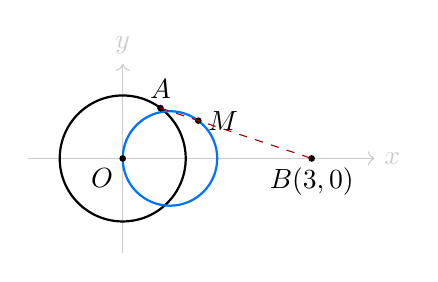
\begin{tikzpicture}[scale=0.8, baseline=(current bounding box.north)]
		\draw[->, gray!40] (-1.5,0) -- (4,0) node[right] {$x$};
		\draw[->, gray!40] (0,-1.5) -- (0,1.5) node[above] {$y$};
		
		% 圆 A (单位圆)
		\draw[thick] (0,0) circle (1);
		
		% 轨迹圆 M
		\draw[thick, SkyBlue] (0.75,0) circle (0.75);
		
		% 点
		\coordinate (B) at (3,0);
		\coordinate (A) at (0.6, 0.8); % 在单位圆上
		% M = 0.75*A + 0.25*B
		\coordinate (M) at ({0.75*0.6 + 0.25*3}, {0.75*0.8}); 
		
		\fill (0,0) circle (1.5pt) node[below left] {$O$};
		\fill (B) circle (1.5pt) node[below] {$B(3,0)$};
		\fill (A) circle (1.5pt) node[above] {$A$};
		\fill (M) circle (1.5pt) node[right] {$M$};
		
		\draw[dashed, DarkRed] (A) -- (M) -- (B);
	\end{tikzpicture}
\end{minipage}

\end{document}